\documentclass[10pt, b5paper]{book}

\usepackage{amsfonts}
\usepackage{amsmath}
\usepackage{amsbsy}
\usepackage{amssymb}
\usepackage{mathrsfs}
\usepackage[left=2.5cm,right=2.5cm,top=3cm,bottom=2.5cm]{geometry}
\usepackage{graphics}
\usepackage{graphicx}
\usepackage{pstricks}
\usepackage{tikz}
\usepackage{caption}
\usepackage[titletoc]{appendix}
\usepackage{wrapfig}
\usepackage{enumitem}

\newcommand{\R}{\mathbb{R}}
\newcommand{\Z}{\mathbb{Z}}
\newcommand{\bigo}{\mathcal{O}}
\newcommand{\st}{\text{fix}}
\renewcommand{\vec}{\mathbf}
\newcommand{\matrx}{\mathbf}
\newcommand{\vecs}{\boldsymbol}
\newcommand{\fourier}{\widetilde}

\renewcommand{\d}{\mathrm{d}}


\newenvironment{exerciseregion}{
  \par\medskip
  \noindent \centerline{\rule{5cm}{1.pt}}
}{\medskip }

\newenvironment{theorem}[1][]{
  \par\medskip  \noindent \textit{Theorem} \rmfamily
} {$\circ$\par\medskip}

\newenvironment{proof}[1][]{
  \par\medskip  \noindent \textit{Proof} \rmfamily
} {$\bullet$\medskip}


\newcounter{example}%[section]
\newenvironment{example}[1][]{\refstepcounter{example}\par\medskip
  \noindent \textbf{Example~\theexample #1} \rmfamily}{$\diamond$\medskip}

%\newcounter{question}%[section]
%\newenvironment{question}[1][]{\refstepcounter{question}\par\medskip
%   \noindent \textbf{Question~\thequestion #1} \rmfamily}{\medskip}

\newenvironment{question}{
  \par\medskip
  \noindent \textbf{Question} \rmfamily
}{\medskip}

\newcounter{exploration}%[section]
\newenvironment{exploration}[1][]{\refstepcounter{exploration}\par\medskip
   \noindent \textbf{Exploration~\theexploration #1} \rmfamily}{\medskip}

 \newcounter{exercise}%[section]
\newenvironment{exercise}[1][]{\refstepcounter{exercise}\par\medskip
   \noindent \textbf{Exercise~\theexercise #1} \rmfamily}{\medskip}


\title{A note on the Reaction-Diffusion Equation}
\author{Jesper S. Hansen}
\date{Fall 2024}

\begin{document}
\maketitle


\begin{center}{\Large{\textbf{Preface to note}}}\end{center}

\bigskip 

\noindent One purpose of mathematical modelling is to obtain a deeper understanding of 
a system or phenomenon. 
The new insight will, hopefully, enable more precise system predictions and control. 
Mathematical modelling can also motivate one to acquire new mathematical skills, and this gives rise 
to explorations of fundamental mathematics. 

This text seeks to give an introduction to mathematical modelling of reaction-diffusion systems. The focus is on 
phenomenology and not on providing detailed quantitative models of specific problems. In the exploration we will 
need and therefore require skills of 
\begin{itemize}
	\item boundary value problems,
	\item the regular perturbation method,
	\item Fourier series and the Fourier transform,
	\item the diffusion equation (example of a parabolic differential equation),
	\item and some particular techniques to analyse the reaction-diffusion equation.
\end{itemize}
The last point includes simple numerical analysis: the numerical algorithms are 
found in the appendices and code can downloaded from the course moodle webpage.  

There are, of course, many different ways we can approach our exploration, but 
there are some obvious choices based on \emph{the principle of progression}. For example, we can 
use some important results from pure diffusion problems to solve the linear reaction-diffusion equation, hence, it 
will be meaningful to treat the former first. On this basis, the text is based on three 
main topics, namely,  
\begin{center}
	the steady state $\rightarrow$ the diffusion equation $\rightarrow$ the
	react. diff. equation.	
	\begin{tikzpicture}
		\draw(1,0.5) -- (1,0);
		\draw(1,0) -- (9,0.0);
		\draw[->](9,0.0) -- (9,0.5);
	\end{tikzpicture}
\end{center}
The arrows indicate depedendencies. 

Our treatment is based on examples, questions, exercises, and, to some extend, proofs of theorems. It is not 
the purpose here to give a formal theoretical foundation of the different topics; this calls for a much more 
rigourus approach and require advanced knowledge of, for example, series convergence and functional analysis.  
The theorems will therefore often only require so-called mild conditions and the proofs will be of the "calculus"-type. 
In this way, the note follows the standard format for many popular texts on mathematical biology.  
I will refer the interest reader to the more advanced literature whenever I can. 

The prerequisite needed to read the note is knowledge of (i) ordinary differential 
equations and initial value problems, (ii) dynamical systems analysis (e.g. phase portrait analysis), 
and (iii) calculus and basic linear algebra. 




\clearpage

\tableofcontents


\chapter{Introduction}


We dive right in: Consider a thin tube of length $L$ with longitudinal axis parallel
with the $x$-axis as shown in Fig. \ref{fig:flux}. Inside
the tube there is a bio-chemical substance, $S$, and  the concentration (or density) of $S$ we denote 
$c$, which is a function of position, $x$, and time, $t$. The fundamental research question 
throughout this text is
\begin{center}
	\emph{how does the function $c=c(x,t)$ evovle in space and time  
	considering diffusion and reaction processes?}
\end{center}
Why this question is interesting in the first place wil hopefully be clear
as we explore the topic in this and the following chapters. Now, 
the first step in the exploration is to derive the underlying dynamical equation for $c$.

\begin{figure}[b]
	\begin{center}
		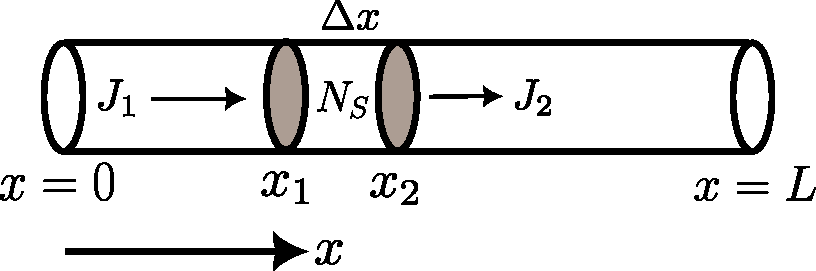
\includegraphics[scale=0.5]{figs/fluxIllustration.pdf}
		\caption{\label{fig:flux}
		Schematic illustration of the effective one dimensional tube system. See the text for 
		explanation of the symbols.
		}
	\end{center}
\end{figure}

We focus on the system volume confined between $x_1$ and $x_2$ and define the 
volume width $\Delta x = x_2 - x_1$. By the \emph{flux} at $x_1$, denoted
$J_1$, we mean the amount of $S$ leaving or entering the volume at $x=x_1$ per
unit time. Likewise, the flux $J_2$ is the amount of $S$ leaving or entering the
volume at $x=x_2$. We ignore any radial and angular fluxes; we call this an effective 
one dimensional system.

There is an important convention here: A flux is positive when the substance flows to the
right (in the ``positive'' $x$-direction) and it is negative if it flows to the
left (``negative'' $x$-direction). 

$S$ can also be produced or consumed inside the volume, for example, through bio-chemical processes. 
The production (or consumption) per unit time we denote $\Delta \sigma$. 
If $N_S$ is the total amount of $S$ in the volume the rate of change of $S$ in the volume is written as
\begin{eqnarray}
	\frac{\d N_S}{\d t} &=& \mathrm{production} + \mathrm{flux \ at} \ x_1 -
	\mathrm{flux \ at} \ x_2 \nonumber \\
	&=& \Delta \sigma + J_1 - J_2 \, . \label{eq:balance}
\end{eqnarray}
This equation is the \emph{balance equation} for the volume. The amount of $S$ at any time is 
\begin{equation}
	N_S(t) = A \Delta x c_s(t) \ \ \mathrm{implying} \ \ \frac{\d N_S}{\d t} = A \Delta
	x \frac{\d c_s}{\d t} \, ,
\end{equation}
where $c_s$ is the average concentration in the volume, and $A$ is the tube cross section area. 
Substitution into Eq.~(\ref{eq:balance}) and dividing with the slab volume $A \Delta x$ we get
\begin{equation}
	\frac{\d c_s}{\d t} = \frac{\Delta \sigma}{A \Delta x} - \frac{1}{A} \frac{J_2
	-J_1}{\Delta x} \, .
\end{equation}
In the limit $\Delta x \rightarrow 0$ we get, now highlighting the time dependence 
\begin{equation}
	\frac{\d}{\d t} c_s(t) = f_s(t) - \frac{\d}{\d x}J_s(t) \, . 
\end{equation}
Here $f_s$ is the production rate per unit volume inside the volume, and $J_s$ is
the net flux per unit area
\begin{equation}
	\frac{\d  J_s}{\d x} = \frac{1}{A}\lim_{\Delta x \rightarrow 0} \frac{J_2-J_1}{\Delta x} \, .
\end{equation}
This must be true for any infinite small volume we consider, thus, for any interior point $x \in ]0; L[$
we can write the balance equation as
\begin{equation}
	\label{eq:reacflux}
	\frac{\partial}{\partial t} c(x,t)= f(x,t) - \frac{\partial}{\partial x}J(x,t)
	\,  .
\end{equation}
For the balance equation, Eq. (\ref{eq:reacflux}), to be meaningful we assume
that both $c$ and $J$ have partial derivatives in their domain; unless otherwise
stated we will make an even more strict assumption that both functions are
differentiable. We here referre to $f$ as the \emph{production function} and $J$ 
simply as the \emph{flux}.

Equation (\ref{eq:reacflux}) formalizes that the local rate of change of
the concentration of $S$ is due to (i) a production process and (ii) how much
substance flows in and out of any point along the tube. As it stands it does not
form a closed problem, since we do not know $f$ or $J$; these we must model.

We often, but not always, let the production be due to bio-chemical reactions. These reactions depend on the 
concentration, i.e., we can write the production function as $f(x,t) = r(c(x,t))$. 

In general, the flux $J$ can be decomposed into a term due to \emph{advection} and a
term due to \emph{diffusion}. Advection is the process that transport a substance
around the system when there is a bulk flow; we will not consider this process. 
Diffusion is the process that tends to remove any gradient in the system:
If you add a drop of dye to a glass of water the colored dye molecules will
eventually distribute uniformly in the system. Therefore, we must intuitively
expect that the flux due to diffusion is non-zero whenever there exists a
gradient in the concentration. This is expressed in \emph{Fick's first law}
\begin{equation}
	J = -D\frac{\partial c}{\partial x} \, .
\end{equation}
Here $D > 0$ is the diffusion coefficient, which in general is dependent on
temperature, position, and so forth.

If we substitute $f(x,t)=r(c)$ and Fick's law into Eq. (\ref{eq:reacflux}) we
get the \emph{reaction-diffusion equation}
\begin{equation}
	\label{eq:reacfdif0}
	\frac{\partial c}{\partial t}= r(c) + \frac{\partial}{\partial
	x}\left[D\frac{\partial c}{\partial x} \right] \, . 
\end{equation}
We abbreviate the reaction-diffusion equation by \emph{RD-equation}. If the
diffusion coefficient is constant the RD-equation becomes
\begin{equation}
	\label{eq:reacfdif1}
	\frac{\partial c}{\partial t}= r(c) + D\frac{\partial^2 c}{\partial
	x^2} \, . 
\end{equation}
Importantly, Fick's law is a \emph{model} and it is therefore, perhaps, unfortunate that
the literature refers to this is a ``law'' \footnote{The same can be said about
Ohm's law, but \emph{not} e.g. Newton's second law}. It proposes that the flux
is linearly dependent on the substance concentration gradient; it must therefore
be considered as the linear term in a Taylor expansion with respect to the gradient, 
and is only usable for sufficiently small gradients (actually, often for surprisingly large
gradients). By the way, this type of model is more formally referred to as a 
\emph{linear constitutive relation}.

\begin{example}
	\label{ex:simplegrowth}
	An important example we will investigate throughout the text is the case of 
	a simple linear growth rate of, say, some biological organism like plankton. 
	In addition to growth, we also include the effect of diffusion in one direction 
	(we have the plankton in a small radius tube). If $c$ denotes the 
	organism concentration and if the diffusion coefficient is constant we have from
	Eq. (\ref{eq:reacfdif1})
	\begin{equation}
		\label{eq:linrd}
		\frac{\partial c}{\partial t} = kc + D \frac{\partial^2 c}{\partial x^2} \, ,
	\end{equation}
	where $k$ is the growth rate coefficient. If the plankton multiply $k>0$; if it
	dies out $k<0$. This RD-equation is a linear differential equation and
	we should be optimistic about finding a solution.

	The RD-equation must be solved by specifying both an \emph{initial condition} (IC) and
	\emph{boundary conditions} (BCs). If the organism at time zero is bundled up at some
	interior point $x_0$, we may specify the IC as a Gaussian shaped curve 
	\begin{equation}
		c(x,0)=c_0 e^{(x-x_0)^2/\sigma^2} \ ,
	\end{equation}
	where $c_0$ is the maximum concentration and $\sigma$ determines the width of
	the Gaussian curve. If we somehow can control the concentrations at the tube
	ends $x=0$ and $x=L$ such that it is zero at these points, we write the BCs as
	\begin{equation}
		\label{eq:bcDiriclecht}
		c(0, t) = 0 \ \ \text{and} \ \ c(L,t) = 0 \ \ \text{for} \ \ t>0 \, . 
	\end{equation}
	These two BCs define a specific function value at the system end-points, and
	are called \emph{Dirichlet boundaries} or boundaries of first type. In general, the
	boundary value can take any (real) value and not just zero. The boundary at $x=0$ we 
	will referre to as the \emph{left boundary} and the boundary at $x=L$ 
	\emph{the right boundary}. 

	Another commonly used BC is the \emph{Neumann boundary}, or boundary of the second
	type. This specifies the values for the function derivatives at the wall, for
	example, 
	\begin{equation}
		\label{eq:bcNeumann}
		\left.\frac{\partial c}{\partial x}\right|_{x=0} = 0
		\ \ \text{and} \ \
		\left.\frac{\partial c}{\partial x}\right|_{x=L} = 0
		\ \ \text{for} \ \ t>0 \, . 
	\end{equation}
	We can also encounter systems with \emph{mixed} BCs, such that at, say, the left boundary we have
	a Neumann BC and at the right boundary we have a Dirichlet BC
	\begin{equation}
		\left.\frac{\partial c}{\partial x}\right|_{x=0} = 0
		\ \ \text{and} \ \
		c(L,t) = C_L  \ \ \text{for} \ \ t>0 \, .
	\end{equation}
	We shall see that the BCs not only determine the solution to a given
	RD-equation, but also determine whether a solution exists or not.
\end{example}


\begin{question}
	What is the bio-physical interpretation of the Neumann BC given in
	Eq.~(\ref{eq:bcNeumann})? 
\end{question}

\begin{example}\label{example:flow}

	\begin{wrapfigure}{R}{0.35\textwidth}
		\centering
		\includegraphics[width=0.3\textwidth]{figs/poiseuille.eps}
		\caption*{}
	\end{wrapfigure}
	\paragraph{}
	\vspace*{-\parskip}

	The mathematical form of the RD-equation is the same as the equation used to describe some 
	special fluid flows. Let a fluid be confined
	between two parallel walls located at $x=0$ and $x=L$. The flow in the
	$y$-direction denoted $v$ is given by the Navier-Stokes equation which
	for sufficiently small flow rate reads
	\begin{equation}
		\frac{\partial v}{\partial t} = g + \nu_0 \frac{\partial^2 v}{\partial
		x^2} \, ,
	\end{equation}
	where the production function $g$ is the local applied accelaration (gravity) and $\nu_0$ 
	the kinematic viscosity.

	In a Couette flow we ignore the applied acceleration $g=0$, and we move one wall with a
	speed $V_0$ while keeping the other fixed. This gives Dirichlet BCs, for example,  
	\begin{equation}
		v(0,t)=0 \ \ \text{and} \ \ v(L,t)=V_L \, .
	\end{equation}
	In a Poiseuille flow we apply an acceleration $g > 0$, but keep the walls
	fixed given raise to the BCs
	\begin{equation}
		v(0,t)=0 \ \ \text{and} \ \ v(L,t)=0 \, .
	\end{equation}
\end{example}

\begin{example}
	\label{example:turing}
	In bio-chemical reactive systems there will be more than just one animal species,
	organism, or chemical compound that multiply, die, or react. In general, there will
	be very many "substances", $S_1, S_2, \ldots$, and the corresponding 
	concentrations, $c_1, c_2, \ldots$,  will be coupled (or co-depended).
	For example, if we wish to model the population of a predator we
	usually also need to include the food resources (prey) unless it is abundant and can be considered 
	constant. The prey dynamics itself depends on the predator population as prey is eaten/consumed 
	by preditors, hence, the two are coupled.

	If we have two coupled concentrations, and assume that diffusion of $c_1$ depends on the gradient 
	of $c_1$ only (and the same for $c_2$) we can write a system of RD-equations 
	\begin{eqnarray}
		\frac{\partial c_1}{\partial t} &=& r_1(c_1,c_2) + D_1 \frac{\partial^2
		c_1}{\partial x^2} \\
		\frac{\partial c_2}{\partial t} &=& r_2(c_1,c_2) + D_2 \frac{\partial^2
		c_2}{\partial x^2} 
	\end{eqnarray}
	In short-hand vector notation we write this as 
	\begin{equation}
		\frac{\partial \mathbf{c}}{\partial t} = \mathbf{R}(\mathbf{c}) + \mathbf{D}
		\cdot \frac{\partial^2 \mathbf{c}}{\partial x^2} \ ,
	\end{equation}
	where $\mathbf{c}=(c_1, c_2)$, $\mathbf{R}$ is a vector-valued reaction function 
	$\mathbf{R} = (r_1, r_2)$ and $\mathbf{D}$ is the so-called diffusion
	matrix
	\begin{equation}
		\mathbf{D} =
		\begin{bmatrix}
			D_1 & 0 \\
			0 & D_2 
		\end{bmatrix} \, .
	\end{equation}
	To proceed we again need to model the reaction terms $r_1$ and $r_2$, as well
	as define the IC and BCs for both concentrations $c_1$ and $c_2$.

	\begin{figure}[t]
		\begin{center}
			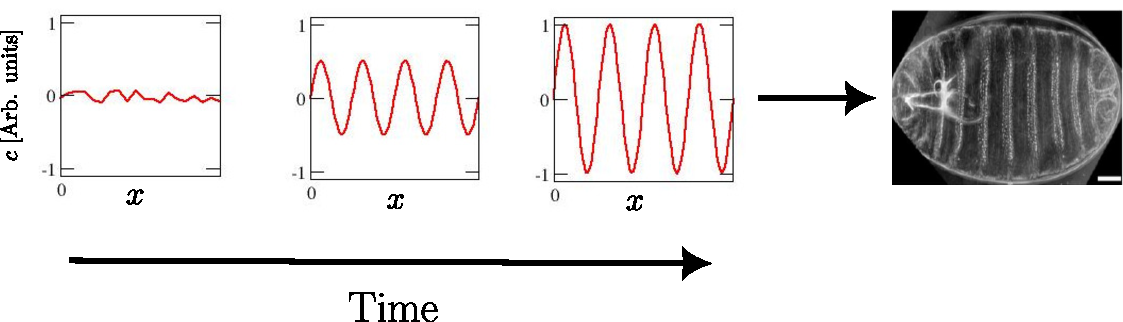
\includegraphics[scale=0.6]{figs/turingIllustration.pdf}
			\caption{\label{fig:turing} Turing structure. From random initial
			concentration (a), a concentration gradient emerges (b), reaching a
			static structure (c).  The Turing structure can model the 
			biological morphology observed in the embryo of the fruit fly (d).  }
		\end{center}
	\end{figure}

	Alan Turing was the first to apply this type of model to account for
	\emph{biological morphology}, that is, what appears to be spontaneously emerging
	structures in biological systems. If the system is initialized in a random 
	(macroscopically uniform) fashion, see Fig. \ref{fig:turing}, then
	concentration gradients emerge spontaneously giving raise to a static (time independent) 
	structure with respect to the concentrations.
\end{example}

\begin{example}
	\label{ex:bacteria-in-dish}
	In the laboratory bacteria can be grown by seeding a small amount of bacteria onto 
	a surface with nutrients and agar (an algae); often this is done in a Petri dish. As the 
	bacteria multiply the colony grows radially from the seeding point.   
	\begin{wrapfigure}{L}{0.35\textwidth}
		\centering
		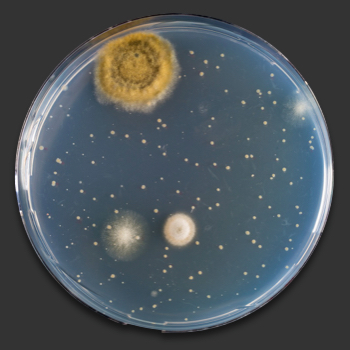
\includegraphics[width=0.3\textwidth]{figs/petri-dish-bacteria-growth.jpg}
		\caption*{}
	\end{wrapfigure}
	\paragraph{}
	\vspace*{-\parskip}
	The growth happens in two spatial dimensions which we can highlight by
	writing  
	\begin{eqnarray}
		c = c(x,y,t) \, .
	\end{eqnarray}
	We must extend the balance equation to describe this situation. 
	In order not to get side tracked, we shall not
	do a formal generalization of the balance equation, but simply give an
	intuitive explanation. In two dimensions the flux occurs in two directions
	and the flux is therefore in general a vector quantity, $\vec{J}=(J_x, J_y)$. 
	Now, as it was the case for one dimension the rate of change of $c$ at a 
	given point depends on the flux in and out of the point, that is,
	it depends on the spatial derivatives of $\vec{J}$. If there is a positive 
	flux in the $x$-direction, but a corresponding negative flux in the
	$y$-direction we must expect the net flux to be zero. This sum (a scalar) 
	is the	\emph{divergence} of $\vec{J}$
	\begin{equation}
		\vecs{\nabla} \cdot \vec{J} = 
		\left( \frac{\partial}{\partial x}, \frac{\partial}{\partial y}\right)
		\cdot (J_x, J_y) = 
		\frac{\partial J_x}{\partial x} + \frac{\partial J_y}{\partial y} \, .
	\end{equation}
	$\vecs{\nabla}$ is denoted the \emph{del operator}. If the divergence is
	positive there exists a net flux out of the point and, vice-versa, if it is 
	negative there is a net flux to the point.  The balance then becomes
	\begin{equation}
		\frac{\partial c}{\partial t} = f(x,y,t) - \vecs{\nabla} \cdot \vec{J} \, . 
	\end{equation}
	Fick's law is in this case is the \emph{gradient} of $c$
	\begin{equation}
		\vec{J} = -D \left(\frac{\partial c}{\partial x}, \frac{\partial
		c}{\partial y}\right) = -D \vecs{\nabla} c \, .
	\end{equation}
	Notice that the gradient $\vecs{\nabla} c$ is a vector. Inserting Fick's
	law into the balance equation we obtain
	\begin{eqnarray}
		\frac{\partial c}{\partial t} &=& f(x,y,t) + \vecs{\nabla} \cdot D
		\vecs{\nabla} c \nonumber \\
		&=&  f(x,y,t) + D \left( \frac{\partial}{\partial x},
		\frac{\partial}{\partial y}\right) \cdot 
		\left(\frac{\partial c}{\partial x}, \frac{\partial c}{\partial y}\right)
		\nonumber  \\
		&=& f(x,y,t) + D \left(\frac{\partial}{\partial x}\frac{\partial c}{\partial x}
		+ \frac{\partial}{\partial y}\frac{\partial c}{\partial y} \right) \nonumber \\
		&=& f(x,y,t) + D \vecs{\nabla}^2 c
	\end{eqnarray}
	if the diffusion coefficient is constant. The second order differential operator 
	\begin{equation}
		\vecs{\nabla}^2 =  
		\left(\frac{\partial^2}{\partial x^2} + \frac{\partial^2}{\partial y^2}
		\right)
	\end{equation}
	is called the \emph{Laplace operator}
	\footnote{and is often (especially among mathematicians) given the symbol $\Delta$}. 

	We return to the bacteria colony. The colony grows radially from a point and
	the Cartesian coordinates above are rather inconvenient to describe this. Rather
	we choose polar coordinates such that
	\begin{eqnarray}
		 c = c(r, \theta, t) \, ,
	\end{eqnarray}
	where $r$ is the radial distance to the seeding point and $\theta$ the polar
	angle. Recall that the relation between Cartesian and polar coordinates are
	\begin{eqnarray}
		x = r \cos(\theta) \ \text{and} \   y = r \sin(\theta) \, .
	\end{eqnarray}
	By heavy usage of the chain rule we can use these relations to derive the 
	Laplace operator in polar coordinates
	\begin{eqnarray}
		\vecs{\nabla}^2 = \left(\frac{1}{r}\frac{\partial}{\partial r}
		r\frac{\partial }{\partial r}  +
		\frac{1}{r^2}\frac{\partial^2}{\partial \theta^2}\right) \, .
	\end{eqnarray}
	An interesting case to us is when the concentration is angle
	independent, $c= c(r,t)$, then the RD-equation reads 
	\begin{equation}
		\label{eq:rdpol}
		\frac{\partial c}{\partial t} = r(c) +
		\frac{D}{r}\frac{\partial}{\partial r}
		\left(  r\frac{\partial c}{\partial r} \right) 
	\end{equation}
	if $D$ is constant and if the production function is $r(c)$. In the reminder of the text we will 
	use one dimensional Cartesian coordinate unless otherwise stated. Only a few
	exercises deal with Eq. (\ref{eq:rdpol}).
\end{example}	

\begin{question}
	What would be appropriate BCs for the bacteria growth in a Petri dish?
\end{question}

\noindent The \emph{steady state} is the state where the system is independent
of time, i.e., the situation where 
\begin{equation}
	\frac{\partial c}{\partial t} = 0 \, .
\end{equation}
This means we can think of $c$ as a function of only the spatial coordinate, 
$c = c(x)$, and results in an ordinary second order differential equation on the form
\begin{equation}
	\label{eq:bcIntro}
	D\frac{\d^2 c}{\d x^2} + r(c) = 0 \, ,
\end{equation}
if the diffusion coefficient is constant. The solution is dependent on the specific BCs, 
and Eq. (\ref{eq:bcIntro}) together with the BCs define a 
\emph{boundary value problem}. In the next chapter we will explore these problems; both in the linear case and 
non-linear case using perturbation methods. 

The diffusion equation represents the case where the reaction (or more generally the 
production function, $f$) is 
absent. The dynamics of $c=c(x,t)$ is then
\begin{equation}
	\frac{\partial c}{\partial t} = D \frac{\partial^2 c}{\partial x^2} 
\end{equation}
for constant diffusion coefficient. This is a 
\emph{parabolic partial differential equation}, and to solve this we need both ICs 
and BCs. In our analysis of this equation it is very 
useful to apply our knowledge of Fourier series and, in particular,  
the Euler-Fourier equations, which we will revisit.

Once we are familiar with the steady state and pure diffusion cases we can explore the full 
RD-equation. Here we will see examples of the linear RD-equation, propagting concentration waves, and Turing 
structures as models for different bio-chemical systems.

This primer on the RD-equation is not meant as a rigorous mathematical treatment, and we approach the topic 
in a rather informal and intuitive manner with examples and excercises supported by computer simulations. 
For a formal treatment, the reader can consult books by 
Grindrod \emph{The Theory and Applications of Reaction Diffusion Equations: Patterns and Waves}
and Smoller \emph{Shock, Waves, and Reactions - Diffusion Equations}.  




%\clearpage

\chapter{The steady-state: Boundary value problems\label{sect:BV}}

An important class of problems deal with the steady-state, i.e., where the
system after a transient time no longer evolves. The steady-state we formally
define as  
\begin{equation}
  \frac{\partial c}{\partial t}=0 
\end{equation}
implying that $c=c(x)$. In this case and for constant diffusion coefficient,
the RD-equation reduces to an ordinary differential equation
\begin{equation}
  D\frac{\d^2c}{\d x^2} + r(c)=0  
\end{equation}
This equation together with some appropriate BCs 
define a boundary value problem and is what we will study in the next few
sections. In the last optional section we explore \emph{chemotaxis} which is a phenomenon where 
cells migrate due to a signaling compound. While this is not a 
reaction-diffusion phenomenon, we can easily apply what we 
learn in the first sections and thus further extent the applications.

The boundary value problems we encounter here when $r$ is a linear function 
are examples of the \emph{Sturm-Liouville} problem. The theoretical 
framework of this general problem is very elegant and quite useful, however, we shall 
not embark on an indepth treatment here, but simply make a few references. 


\section{Linear reaction functions \label{stst:sectBVP}}
In Example \ref{ex:simplegrowth} we 
introduced an RD-equation with a simple linear reaction function, $r=kc$.  
Let us explore this example in the case where $k>0$, that is, the population
self-multiply,  
\begin{equation}
  \label{eq:simplegrowthss}
	D\frac{\d^2c}{\d x^2} + kc=0 \, \ \ \ (k>0).
\end{equation}
Since we have no time in the problem we do not have an IC, and in this first
example we apply simple Dirichlet BCs
\begin{equation}
  c(0)=c(L)=0 \, .
\end{equation}
The general solution to this homogeneous second order linear equation with
constant coefficients depends on the eigenvalues' multiplicity 
\footnote{If you need to refresh this, I recommend the book 
by Boyce \& DiPrima, \emph{Elementary Differential Equations}, 
published by Wiley.}. To find this, we can write the characteristic polynomial for
Eq. (\ref{eq:simplegrowthss}) 
\begin{equation}
	\lambda^2 + \frac{k}{D} = 0 \ \Rightarrow \ \lambda_{1,2} = \pm i \sqrt{\frac{k}{D}}   \, ,
	 \label{eq:eigInfinite}
\end{equation}
where $\lambda$ is the \emph{eigenvalue}. Since the multiplicity is one 
(for both eigenvalues, of course) the general solution is 
a linear combination of two exponential functions. Applying Euler's identity we get
\begin{eqnarray}
  c(x) &=& A e^{i \sqrt{k/D} x} + B e^{-i \sqrt{k/D} x}
           \nonumber \\
       &=& (A+B)\cos\left(\sqrt{k/D}\,x\right) +
           i(A-B)\sin\left(\sqrt{k/D}\,x\right) \, ,
		   \label{eq:stsgeneral2order}
\end{eqnarray}
where $A$ and $B$ are constants we must seek from the BCs. 

From the left BC (at $x=0$) we get
\begin{equation}
  c(0) = A + B = 0 \ \Rightarrow \ A = -B   \, ,
\end{equation}
and using this result together with the right BC (at $x=L$)
\begin{equation}
  c(L) = i2A\sin\left(\sqrt{k/D}\,L\right) = 0 \, .
\end{equation}
This relation is of course fulfilled for $A=0$ and this leads to the 
\emph{trivial solution} $c(x)=0$. Perhaps more interestingly, the equation is also 
fulfilled for $A\neq 0$ and $\sin(\sqrt{k/D}\,L ) = 0$, that is, for
\begin{equation}
  \label{eq:constraintL}
	\sqrt{\frac{k}{D}} \, L = n\pi \, , \ \text{where} \ n \in \mathbb{N}_+ \, .
\end{equation}
Since $k, D$ and $L$ are all larger than zero, the right-hand side must be positive 
implying that $n$ is a positive integer as we indicate by $\mathbb{N}_+$. 

Rearranging Eq.(\ref{eq:constraintL}) 
and substituting into the general solution, Eq. (\ref{eq:stsgeneral2order}), we have
that   
\begin{equation}
\label{eq:gensolfirst}
c(x) = i2A \sin\left(\frac{n \pi}{L} \, x \right) \, \ \text{for any} \ n \in \mathbb{N}_+ \, .
\end{equation}
In our treatment here, $c$ is a real valued function and therefore $A$ must be imaginary. Also, if 
we demand $c \geq 0$ ($c$ representing concentration) only $n=1$  will work, defining the length    
\begin{equation}
  \label{eq:L0}
  L_0 = \pi  \sqrt{\frac{D}{k}} \, ,
\end{equation}
constraining the $x$-coordinate to $0 \leq x \leq L_0$. 

Even if we have two BCs we cannot determine the constant $A$ (and get a unique solution for 
the special case $n=1$). What we got from the BCs is the relation between the constants $A$ and $B$, 
and the non-trivial solution constraint given in Eq. (\ref{eq:constraintL}). 
We must conclude that there exists infinitely many solutions. 

The result here, namely, that there does not exists a unique solution may be 
surprising if we consider the corresponding
experimental bio-chemical system we seek to model. The substance (here a plankton population)
features a self-multiplying process, and due to the concentration gradient,
the produced plankton is transported via diffusion to the tube-ends where it is
removed (how, will not concern us here). Now, if the diffusion transport 
is sufficiently fast compared to the production, the population vanishes with time 
(as the plankton is removed at the tube ends), and we simply end in the trivial solution $c=0$. 
On the other hand, if diffusion cannot transport the produced plankton to the tube ends fast enough, the concentration
will keep raising leading to $c$ diverging at all interior points; and now we must of course evaluate whether our
model fulfill its purpose. Finally, there is also a state where there exists a 
(fragile) balance between the diffusive transport out of the system 
and the production allowing for a non-trivial solution. \label{page:nouniquness} In Chapter \ref{ch:rd} we revisit these points in more detail. 

Let us briefly return to the solutions in Eq. (\ref{eq:gensolfirst}). The \emph{super-position principle for linear systems} 
states that if Eq. (\ref{eq:gensolfirst}) are solutions to the problem, then a
linear combination of these solutions is also a solution. Therefore, we also
have, in general, the series solution
\begin{equation}
	\label{eq:2ndorderseries}
	c(x) = \sum_{n=1}^\infty b_n \sin\left(\frac{n\pi}{L} \, x \right) \, ,
\end{equation}
where $b_n \in \R$ a constants. We shall use this important result later.

\begin{question}
	Can you prove the statement in Eq. (\ref{eq:2ndorderseries})? (That is, show
	Eq. (\ref{eq:2ndorderseries}) is solution to Eq. (\ref{eq:simplegrowthss})
	with the BCs $c(0)=c(L)=0$.)
\end{question}

Some terminology: We can rewrite the relation in Eq. (\ref{eq:constraintL}) slightly 
\begin{eqnarray}
	\sqrt{\frac{k}{D}} = \frac{n\pi}{L} \, .
\end{eqnarray}
Comparing this with Eq. (\ref{eq:eigInfinite}) this motivates 
us to name $n\pi/L$ an eigenvalue, and we therefore assign it the symbol
$\lambda_n$, where $n$ refers to the natural number in the nominator. 
Note, for this problem we have infinitely many eigenvalues where $\lambda_n < \lambda_m$ 
if $n<m$. \footnote{This result can be proven formally.} The solution for a given 
eigenvalue is called an \emph{eigenfunction}. The trivial solution, $c=0$, is not an eigenfunction. 

Let us see two more examples.

\begin{example}
	In case the production function is a constant we have an inhomogeneous
	equation on the form
	\begin{equation}
		\frac{\d^2c}{\d x^2} = K \ , \ \ K\in \R.
	\end{equation}
	We will apply mixed boundaries
	\begin{equation}
		c(0)=0 \ \ \text{and} \ \ \left.\frac{\d c}{\d x}\right|_{x=L}=1 \, .
	\end{equation}

	\begin{wrapfigure}[15]{L}{0.4\textwidth}
		\centering
		\includegraphics[width=0.35\textwidth]{figs/solutionEx4.eps}
		\caption*{}
	\end{wrapfigure}
	\paragraph{}
	\vspace*{-\parskip}
	The experimental realisation of these BCs is of no importance to us here. 

	Clearly, the exponential function cannot be a solution to this problem. 
	Let $y=\d c/\d x$, then	$\d y/\d x = K$, implying that $y = Kx + A$ and therefore
	\begin{equation}
		c(x) = \frac{K}{2}x^2 + Ax + B \, .
	\end{equation}
	From the left BC we get $B=0$, and since 
	\begin{equation}
	 \left.\frac{\d c}{\d x}\right|_{x=L}= KL + A = 1 \ \Rightarrow \ A = 1 - KL
	\end{equation}
	the solution is 
	\begin{equation}
	\label{eq:solutionEx4}
	 c(x) = \frac{K}{2}x^2 + (1-KL)x 
	\end{equation}
	This was less painful; 
	in summary, the solution exists and is unqiue.   
%	\marginpar{\includegraphics[scale=0.255555]{figs/solutionEx4.eps}}i
\end{example}

\begin{example}
  We again consider the simple linear growth problem 
  \begin{equation}
    D\frac{\d^2c}{\d x^2} + kc=0 \, , 
  \end{equation}
  but this time we will apply the BCs
  \begin{equation}
    c(0) = 1 \ , \ c(L_0) = 1 \, .
  \end{equation}
  $L_0$ is given in Eq. (\ref{eq:L0}).  Now, the general solution is the same
	as above, Eq. (\ref{eq:stsgeneral2order}), 
	and from the first BC we obtain the relation $B=1-A$. From the second BC we have 
  \begin{equation}
    c(L_0)=\cos(\pi) + i(2A-1)\sin(\pi) = -1 \, .
  \end{equation}
	This conflicts with the right BC and is and example of an \emph{ill posed problem}. 
	Both BCs cannot be satisfied and no solution exists.
\end{example}

The examples show that we need to be careful when dealing with boundary
value problems. Even if the differential equation looks harmless and the general
solution exists it may be an ill posed problem or have infinitely many solutions. 
We cannot transfer the results from initial value problems to boundary value
problems. In summary, we have the following possible outcomes:
\begin{itemize}
\item There does not exist a solution.
\item There exists one unique solution. 
\item There exist infinitely many solutions.
\end{itemize}
We will return to existence and uniqueness in the next section.

In this section, we have only dealt with the case where both the
rate constant $k$ and the diffusion coefficient $D$ are true constants and
independent of position. Clearly, this need not to be the case, e.g., 
if the substance is distributed in an inhomogeneous medium. These types of
problems calls for a different approach, which we will see an example of later
in the text.  

\begin{exerciseregion}
  
\begin{exercise}
  Solve the boundary value problems:
  \begin{enumerate}
  \item  
    $\frac{d^2c}{dx^2} = K \ \text{with} \  c(0) =0\, , \ c(L)=0$

   \item 
    $\frac{d^2c}{dx^2} = 0 \ \text{with} \ c(0)=0\, , \ c(L)=C_L $
  \item 
    $\frac{d^2c}{dx^2} = -c \ \text{with} \  \left.\frac{\d c}{\d x}\right|_{x=0} =1\, , \ c(L)=0$
  \end{enumerate}
  Relate 1 and 2 to the flow cases in Example \ref{example:flow}.
\end{exercise}

\begin{exercise}
	\label{exercise:ststneumann}
	(Mandatory) Consider the Neumann boundary value problem
	\begin{eqnarray}
		\frac{\d^2c}{\d x^2} + \alpha c = 0 \ \text{with} \  \left.\frac{\d c}{\d x}\right|_{x=0} = \left.\frac{\d c}{\d x}\right|_{x=L} =0
	\end{eqnarray}
	Show that   
	\begin{itemize}
		\item this problem has no solutions when $\alpha < 0$, 
		\item this problem has infinite many solutions when $\alpha > 0$, and
		\item that the general solution is on the form
		\begin{equation}
			\label{eq:2ndorderseriescosine}	c(x) = \sum_{n=0}^\infty c_n \cos\left(\frac{n\pi}{L} \, x \right) \, ,
		\end{equation}
		where $c_n \in \R$ is a constant.
	\end{itemize}
	 We shall use these important results later. 
\end{exercise}
\begin{exercise}
  Show that when $k<0$ the trivial solution, $c=0$, is a solution to the steady-state
  problem, Eq.(\ref{eq:simplegrowthss}). How do you bio-physically argue that
	this is the only solution?
\end{exercise}

\end{exerciseregion}


\section{Existence and uniqueness of solutions} \label{sect:uniq}
As illustrated in the previous section, we are not guaranteed a unique or even a single solution 
to a given boundary value problem. In some cases we can give a formal proof if a solution exists to 
a given problem and whether it is unique. 

To give an example, consider the famous one dimensional \emph{Laplace equation} 
\begin{equation}
  \label{eq:laplace}
  \frac{\d^2 c}{\d x^2} =  0 \, . 
\end{equation}
 
\begin{theorem}
  The only solution to the Laplace equation with Dirichlet BCs
  \begin{equation}
    c(0) = c(L)=0
  \end{equation}
  is the trivial solution $c=0$.
\end{theorem}
Before going through the formal proof we can quite easily understand why
this is likely true. A good guess for the general solution to the Laplace equation is a
simple linear function on the form $c = ax + b$, where $a$ and $b$
are the coefficients we must find from the BCs. The condition $c(0) = 0$ implies that $b=0$,
and only $a=0$ then satisfies $c(L) = 0$, that is, $c=0$.

\begin{question}
	Why should we not consider this reasoning as a satisfactory proof for existence and uniqueness?
\end{question}

\begin{proof}
	Assume two solutions exists, namely, $\varphi_1$ and $\varphi_2$. We then 
	define a third function, $\varphi$, 
	as the difference $\varphi = \varphi_1 - \varphi_2$, thus, if we can show $\varphi = 0$ we have shown 
	that only one solution exists. Notice that $\varphi$ fulfills the Laplace equation with same 
	Dirichlet BCs as the original problem since
	\begin{equation}
		\label{eq:laplacevarphi}
		 \frac{\d^2 \varphi}{\d x^2} =  \frac{\d^2 \varphi_1}{\d x^2} -  \frac{\d^2 \varphi_2}{\d x^2} = 0   
	\end{equation}
	and $\varphi(0) = \varphi(L)=0$. 

	From the product rule we have the following identity
	\begin{equation}
    	\frac{\d}{\d x}\left(\varphi \frac{\d \varphi}{\d x} \right) = \left( \frac{\d \varphi}{\d
        	x}\right)^2 + \varphi \frac{\d^2 \varphi}{\d x^2} = \left( \frac{\d \varphi}{\d x}\right)^2 \, ,
  \end{equation}
  where the last relation is due to Eq. (\ref{eq:laplacevarphi}). We integrate
	both sides; from the fundamental theorem of calculus the left-hand side
	becomes 
  \begin{equation}
    \int_0^L \frac{\d}{\d x}\left(\varphi \frac{\d \varphi}{\d x} \right) \, \d x  =
    \left.  \varphi \frac{\d  \varphi}{\d x} \right|_{x=0}^{x=L} = 0 
  \end{equation}
  from the BCs. This implies that the right-hand is also zero, i.e.,
  \begin{equation}
	  \int_0^L \left( \frac{\d  \varphi} {\d x}\right)^2 \, \d x = 0  \, .
  \end{equation}
  The integrand is always zero or positive because it is a real function squared, 
	thus, for the integral to be zero we
  must have $\d  \varphi /\d x = 0$ for $0 \leq x \leq L$. The only way the BCs can be
  satisfied is then if
  \begin{equation}
     \varphi  = \varphi(0)= \varphi(L)=0 \ \text{for}  \ 0 \leq x \leq L \, . 
  \end{equation}
	This means that $\varphi_1=\varphi_2$ (only one solution exists), 
	and since $\varphi$ is given by the original Laplace equation we have $\phi=c$ and only the 
	trivial solution is the solution.
\end{proof}

\noindent Things change dramatically if we change the BCs. 
\begin{theorem}
  The Laplace equation with Neumann BCs
  \begin{equation}
    \frac{\d^2c}{\d x^2} = 0 \ , \ \text{with} \  
    \left.\frac{\d c}{\d x}\right|_{x=0}=\left.\frac{\d c}{\d x}\right|_{x=L} =0 \, ,   
  \end{equation}
  does not have a unique solution.
\end{theorem}

\begin{proof}
	The proof follows the same idea as above and is left to the reader 
	(Come to class if you are stuck!)
\end{proof}

Except from the exercises below, we shall not pursue proving these 
existence and uniqueness theorems further in this text; again the 
interested reader can consult the literature on this. 

\begin{exerciseregion}
\begin{exercise}
  Prove that the only solution to the boundary value problem
  \begin{equation}
    \frac{\d^2c}{\d x^2} = c \ , \ c(0)=c(L)=0 \, ,
  \end{equation}
  is the trivial solution.
\end{exercise}

\begin{exercise}
	Prove that the \emph{Poisson equation} with Dirichlet BCs
	\begin{equation}
	  \frac{\d^2c}{\d x^2} = f(x) \ , \ c(0)=c(L)=0 \, ,
	\end{equation}
	has a unique solution. $f$ being some real valued production function.
\end{exercise}

\end{exerciseregion}
 

\section{Non-linear reaction functions}
Bio-chemical reactions are often non-linear. The 
first way to approach such situation is, almost always, to study the
corresponding local linearized system in hope this gives some qualitative
understanding of the system. Some times, however, we wish to extend our analysis, e.g., 
if we want a better quantitative output from the model. 

Consider the steady state problem
\begin{equation}
  D\frac{\d^2c}{\d x^2} + k c^2 = 0 \ \ \text{with} \ \ 
  c(0) = 0 \ \ \text{and} \ \ c(1)=1 \, .
\end{equation}
Notice the reaction term is non-linear and we cannot use the standard
techniques discussed so far to solve this. We can re-arrange this and introduce a 
new parameter $\epsilon = k/D$, $D \neq 0$, 
such that the dynamical equation becomes
\begin{equation}
  \label{eq:second}
  \frac{\d^2c}{\d x^2} + \epsilon c^2 = 0 \, . 
\end{equation}
In cases where diffusion dominates, $D \gg k$, we have that $\epsilon$ is small. 
Indeed, we will expect that the solution in this case 
is ``close'' to the solution for $\d^2c/\d x^2 = 0$,  
where there is no reaction process. We can think of $\epsilon$ as a parameter that controls 
a (small) perturbation of the system away from the pure diffusion case. 
For this reason $\epsilon$ is called the \emph{perturbation parameter} and Eq. (\ref{eq:second}) 
forms a \emph{regular perturbation problem}. A non-regular problem is illustrated later.

Once we have defined a small system parameter and have a regular perturbation problem, 
we can attempt to do an analysis based on the \emph{regular perturbation method}. 
This method is based on the fundamental assumption (ansatz) that the function
$c$ can be represented by power series with respect to the perturbation parameter. 
At first this does not appear to be very helpful since we are interested in $c$ as a
function of the spatial coordinate $x$ and not the parameter $\epsilon$,
however, the power series will result in a, some times, tractable structure. The
regular perturbation method involves the following five steps:


\begin{enumerate}
\item{Assume that a solution $c=c(x)$ exists. Furthermore assume that $c$ can
    be written in terms of a power series with respect to $\epsilon$
    \begin{equation}
      \label{eq:pertass1}
		c(x) = c_0(x) + \epsilon c_1(x) + \epsilon^2 c_2(x) + \epsilon^3c_3(x) + \ldots
    \end{equation}
    where $c_0$, $c_1$, \ldots are functions of $x$ and independent of
    $\epsilon$. We now hope that $c$ is "well-approximated" with only a 
    few terms, that is, we hope that the function series converges to
    the actual function quickly. Below we specify what well-approximated 
	means.
  }
\item{ 
    Insert the power law series for $c$ into the dynamical equation for $c$,
    Eq. (\ref{eq:second}),
    \begin{eqnarray}
      \frac{\d^2}{\d x^2} (c_0 + \epsilon c_1 + \epsilon^2 c_2 + \dots) +
      \epsilon(c_0 + \epsilon c_1 + \epsilon^2 c_2 + \dots)^2 = 0  \, .
    \end{eqnarray}
  }
\item{
    Collect term-wise with respect to powers of $\epsilon$. To fulfill the
	equation we equate all terms with zero, and letting $\epsilon \neq 0$ we
		obtain	
    \begin{eqnarray}
      &\epsilon^0:& \ \frac{\d^2 c_0}{\d x^2} = 0 \label{eq:p1}\\
      &\epsilon^1:& \ \frac{\d^2 c_1}{\d x^2} + c_0^2 = 0  \label{eq:p2}
      \\
      &\epsilon^2:& \ \frac{\d^2 c_2}{\d x^2} + 2c_0c_1 = 0 \\
      &\vdots& \nonumber
    \end{eqnarray}
		We see this results in a set of tractable problems (albeit in general quite tedious).
	    From Eq. (\ref{eq:p1}) we obtain $c_0$
   		(once the appropriate boundary conditions are specified). This
    result is substituted into Eq. (\ref{eq:p2}) and $c_1$ can be found
    (once the appropriate boundary conditions are specified), and so
    forth. Notice that in this case each problem is linear.
  }
\item{
    Solve for $c_0, c_1, \ldots$
    
    Here we first need to define the boundary conditions. We can let the unperturbed
    problem, $\epsilon=0$, fulfill $c(0)=0$ and $c(1)=1$, that is, we must have
    $c_0(0)=0$ and $c_0(1)=1$. This implies that $c_n(0)=0$ and $c_n(1)=0$,
    $n=1,2$,\ldots.

    Then solving
    \begin{eqnarray}
      &\epsilon^0:& \ \frac{\d^2 c_0}{\d x^2} = 0, \
                    c_0(0)=0, c_0(1)=1 \ \Rightarrow c_0(x) = x
                    \label{eq:p11}\\
      &\epsilon^1:& \ \frac{\d^2 c_1}{\d x^2} + x^2 = 0 \
                    c_1(0)=0, c_1(1)=0 \ \Rightarrow c_1(x) = \frac{x-x^4}{12}
                    \nonumber \\ \label{eq:p12}\\
      &\vdots& \nonumber
    \end{eqnarray}
  }
\item{
    Collect the terms in accordance with Eq. (\ref{eq:pertass1}), here
    to first order in $\epsilon$
    \begin{equation}
      c(x) = x + \frac{\epsilon}{12}(x-x^4) + \dots
      \end{equation}
    }
\end{enumerate}    
\begin{wrapfigure}[14] {R}{0.4\textwidth}
	\includegraphics[width=0.35\textwidth]{figs/perturb_one.eps}
	%\caption{\label{fig:img2} Perturbation}
\end{wrapfigure}
\paragraph{}
\vspace*{-\parskip}
This is the solution from the regular perturbation method; we here stop at first order already, but 
one can continue (see the exercises). 

In this example, the first order term, a measure of the effects from the reaction,
has a pre-factor of $\epsilon/12$. Therefore, the reaction process has only a small effect 
on the concentration profile even if $\epsilon$ is much larger than zero (and we move away from 
the regime $D \gg k$). 

The truncated power series above is formally known as the \emph{Poincar\'{e} expansion}, and the 
approximation is written as
\begin{eqnarray}
	c(x) \sim \sum_{n=0}^N \epsilon^n c_n(x)  \, .
\end{eqnarray}
The \emph{remainder} can now be defined as 
\begin{eqnarray}
	R_N(x,\epsilon) = c(x) - \sum_{n=0}^N \epsilon^n c_n(x)  
\end{eqnarray}
and is a measure for the difference between the actual solution and the Poincar\'{e} expansion. Often 
we do not have an analytical expression for $c$ itself, but have to use a numerical computation. 
We can now define what we mean by the term well-approximated that we used 
above: The Poincar\'{e} expansion (with $N$ terms) is an asymptotic approximation to $c$ if for
all $M\leq N$ and $x \in [0; L]$ we have
\begin{eqnarray}
	\lim_{\epsilon \rightarrow 0}	\frac{R_M(x, \epsilon)}{\epsilon^M c_M(x)} = 0  \ 
	\text{for any fixed $x \in [0;L]$} \ .
	\label{eq:asymappr}
\end{eqnarray}
The asymptodic approximation is, likely, 
best illustrated with an example where the solution is known. 
\begin{example}
    The perturbation method is applicable for different types of non-linear
	problems, not only differential equations. Consider the quadratic problem 
	(example from Hince, \textit{Perturbation Methods})
	\begin{equation}
 	 \label{eq:quadratic}
	  c^2 - \epsilon c -1 = 0 \, .
	\end{equation}
	Proposition: The Poincar\'{e} expansion
	\begin{eqnarray}
		c \sim c_0 + \epsilon c_1 + \epsilon^2c_2 
	\end{eqnarray}
	is an asymptodic approximation to the quadratic problem, Eq. (\ref{eq:quadratic}).

	First, the solution is found from the quadratic formula
	\begin{eqnarray}
		\label{eq:solquadratic}
		c = \frac{1}{2} \left(\epsilon \pm \sqrt{\epsilon^2+4}\right) \, .
	\end{eqnarray}
	Notice that for $\epsilon = 0$	we have $x=\pm 1$. 
	Substituting the expansion and collecting the terms we have up to
	second order 
	\begin{eqnarray}
  	&\epsilon^0:& c_0^2 - 1 = 0 \ \Rightarrow \ c_0 = \pm 1 \\
  	&\epsilon^1:& 2 c_0c_1 - c_0= 0 \ \Rightarrow \ 
                \left\{
                \begin{matrix}
                  2c_1-1  = 0 \\
                  -2c_1 + 1 = 0
                \end{matrix}
  \right. \ \Rightarrow \ c_1 = \frac{1}{2} \\
  &\epsilon^2:& 2c_0c_2 + c_1^2-c_1 = 0
                \ \Rightarrow \ 
                \left\{
                \begin{matrix}
                  2c_2- \frac{1}{4}  = 0 \\
                  2c_2 + \frac{1}{4}= 0
                \end{matrix}
  \right. \ \Rightarrow \ c_2 = \pm \frac{1}{8} 
\end{eqnarray}
hence, the roots to second order in perturbation parameter are
	\begin{equation}
	  \pm 1 + \frac{\epsilon}{2} \pm \frac{\epsilon^2}{8} \, . 
	\end{equation}
	We have to show the limits in Eq. (\ref{eq:asymappr}) (noting that $x$ is 
	not in the current problem). 

	For $M=0$ we have $c_0= \pm 1$ and 
	\begin{equation}
		R_0(\epsilon) = \frac{1}{2}(\epsilon \pm \sqrt{\epsilon^2 + 4}) \mp 1
	\end{equation}
	quickly see that
	\begin{eqnarray}
		\lim_{\epsilon \rightarrow 0} \frac{R_0(\epsilon)}{c_0} = \lim_{\epsilon
		\rightarrow 0} \frac{1}{2}(\epsilon \mp \sqrt{\epsilon^2 + 4}) \pm 	1 =
		0.
	\end{eqnarray}
	For $M=1$
	\begin{eqnarray}
		\lim_{\epsilon \rightarrow 0} \frac{R_1(\epsilon)}{\epsilon c_1} 
		=\lim_{\epsilon \rightarrow 0} \frac{\pm \sqrt{\epsilon^2+4} \mp 2}{\epsilon} 
		= \lim_{\epsilon \rightarrow 0} \frac{\epsilon}{\sqrt{\epsilon^2+4}} = 0 \, .
    \end{eqnarray}
	Last limit is found from L'Hopital's rule. Finally, for $M=2$ we have 
	\begin{eqnarray}
		\lim_{\epsilon \rightarrow 0} \frac{R_2(\epsilon)}{\epsilon^2 c_2} 
		= \lim_{\epsilon \rightarrow 0} \frac{\pm 4\sqrt{\epsilon^2 +4} \mp 8 \mp \epsilon^2}{\epsilon^2} 
		= 0 \, ,
	\end{eqnarray}
	applying L'Hoptial's rule twice. Thus, the Poincar\'{e} expansion with $N=2$ is an 
	asymptotic approximation to the quadratic equation, Eq. (\ref{eq:quadratic}). 
\end{example}

\noindent Be aware, the perturbation method may not always
be helpful, at least not without performing additional tricks. Consider a
slightly different quadratic equation from above  
\begin{equation}
  \epsilon c^2 -c -1 = 0 \, .
\end{equation}
(Again, an example from Hince.) We immediately see that when $\epsilon=0$ 
there is only one solution, but for $\epsilon \neq 0$ there are two. 
A problem where the solution
shows such qualitative change setting $\epsilon=0$ is called a
\emph{singular perturbation problem}. Equation (\ref{eq:quadratic}) above 
is a regular perturbation problem since the number of
solutions did not change by varying $\epsilon$ around zero.
Performing the same steps as we did for regular problems,  
some times called \emph{the outer solution} when we deal with singular problems, we end up with the expansion
\begin{equation}
  c = 1 -\epsilon + 2\epsilon^2 + \ldots
\end{equation}
Compare this to the quadratic formula
\begin{equation}
	\label{eq:quadricformulaPerturb}
  c = \frac{1}{2\epsilon}(1 \pm \sqrt{1-4\epsilon}) \ \ \epsilon  \neq 0 \, .
\end{equation}
These are two very different results, and since we trust the latter we must disregard the 
simple Poincar\'{e} expansion. 

Singular perturbation problems are not just far-fetched curiosities. 
Consider the steady-state RD-equation in the reaction dominated regime, $k \gg D$. 
Here we can introduce the perturbation parameter $\epsilon = D/k$ and we can write
\begin{equation}
  \label{eq:second-singular}
  \epsilon \frac{\d^2c}{\d x^2} + c^2 = 0 \, . 
\end{equation}
As $\epsilon \rightarrow 0$ the diffusion term vanishes and the problem is algebraic only 
allowing $c=0$ at $0 < x < L$, that is, the system qualitative behavior changes dramatically as we 
approach the limit $\epsilon \rightarrow 0$i; this is singular perturbation problem. 
We will later encounter such problem, however, the naive outer solution will in
fact be very helpful here.  

\begin{exerciseregion}

\begin{exercise}
  Find the second order perturbation term for the boundary value problem
  Eq. (\ref{eq:second}). Plot $c_0$, $c_1$, $c_2$ as functions of $x$ with some
  chosen values of $\epsilon$.
\end{exercise}

\begin{exercise}
	Taylor expand to second order 
	the exact solution to the quadratic problem, Eq. (\ref{eq:solquadratic}), 
	in terms of $\epsilon$ around $\epsilon=0$. Compare with the perturbation solution. 
\end{exercise}

\begin{exercise}
  Consider the initial value problem
  \begin{equation}
    \frac{\d c}{\d x} - \epsilon c^2 = 0 \ , \ c(1)=1
  \end{equation}
  	Find the analytical solution. Then use regular perturbation method
  up to second order in $\epsilon$ to approximate the solution. Is the 
  Poincar\'{e} expansion with $N=1$ an asymptodic approximation?		
\end{exercise}

\begin{exercise}
  Consider the boundary value problem
  \begin{equation}
    \frac{\d^2 c}{\d x^2} + c - \epsilon c^2 = 0 \ , \ c(0)=c(1)=1
  \end{equation}
  Use regular perturbation method up to second order and find the
  approximate solution...or die trying.
\end{exercise}

\begin{exploration}
  Figure \ref{fig:biopore} illustrates a cylindrical pore embedded in a
  membrane. The pore allows for transport of a chemical signaling compound
  C. In the steady-state, C has concentration $C_0$ on the ``outside'' and $C_1$
  on the ``inside''. Careful measurements have established that $C_1 > C_0$, and
  from this we expect that a reaction inside the pore consumes the chemical
  C. 
	\begin{figure}[h!]
    \begin{center}
      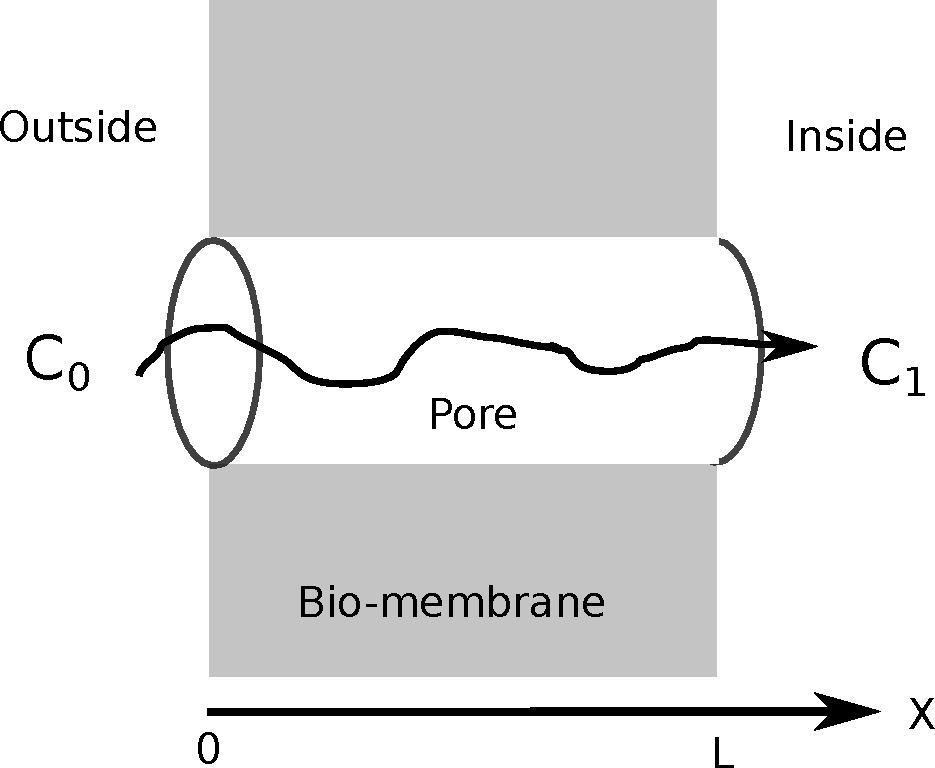
\includegraphics[scale=0.4]{figs/biopore.pdf}
      \caption{\label{fig:biopore}
        Illustration of the bio-pore.
      }
    \end{center}
  \end{figure}
  
  Let the steady-state concentration of C in the pore be denoted $c=c(x)$ where
  $0 \leq x \leq L$. The dynamics is modelled from the steady-state RD-equation
  with mixed BCs
  \begin{equation}
    \label{eq:rdss}
    r(c) + D \frac{\d^2c}{\d x^2} = 0 \ , \ c(0)=C_0 \ \ \text{and} \ \
    \left. \frac{\d c}{\d x}\right|_{x=L} =0 \, .
  \end{equation}
  
  \begin{enumerate}
  \item Show that the condition $C_0 > C_1$ cannot be met if the
    reaction term in Equation (\ref{eq:rdss}) is omitted. 
  \item Show that if $r(c)=-k_1c$ the concentration profile is given by
    \begin{equation}
      c(x) = C_0\left[
        e^{-\alpha L}\frac{\sinh(\alpha x)}{\cosh(\alpha L)} + e^{-\alpha x}
      \right] \, ,
    \end{equation}
    where $\alpha = \sqrt{k_1/D}$
  \item Now let $r(c)=-k_2c^2$. Find the solution up to first order in
    the perturbation parameter $\varepsilon = k_2/D$. Explain the
    fundamental physical unit that determines the validity of this
    approximate solution.
  \end{enumerate}
  \end{exploration}
\end{exerciseregion}

\section{Chemotaxis}
Experimentally it has been observed that some cells, e.g., E-coli, can
register (or sense) 
a chemical concentration gradient and move either down or up this gradient. 
The chemical compound can be a hormone and cell motion 
is realised by, for example, flagella propulsion. 
This phenomenon is denoted \emph{chemotaxis}. To model chemotaxis we need to
change the fluxes in the system. If diffusion and chemotaxis are independent processes we
can write the flux with two terms: (i) a term describing the usual diffusive flux 
and (ii) a term describing the flux due to chemotaxis. 

Consider a cell population with concentration $c_1=c_1(x,t)$ mixed with a
a chemical compound having concentration $c_2=c_2(x,t)$. The \emph{Keller-Segel
model} for the flux of the cells reads
\begin{eqnarray}
	J_1 = \chi c_1 \frac{\partial c_2}{\partial x} - D_1 \frac{\partial c_1}{\partial x} \, ,
\end{eqnarray}
where $\chi$ is the \emph{chemotactic strength} and $D_1$ the usual diffusion 
coefficient for the cells. What the two terms describe should be clear. If the chemotactic strength 
or the gradient of the chemical is zero, then, of course, no flux occurs due to chemotaxis. 
The product in the chemotaxis term between $c_1$ and $\partial c_2/\partial x$ give raise to a 
(potential) non-linearity, and ensures that there is no flux of cells at point when there are no
cells even if the gradient of the chemical is non-zero. Substitution into the 
balance equation for $c_1$ gives 	
\begin{eqnarray}
	\frac{\partial c_1}{\partial t} = r(c_1) - \chi \frac{\partial}{\partial x} \left( c_1 \frac{\partial c_2}{\partial x} \right)
	+ D_1 \frac{\partial^2c_1}{\partial x^2} 
\end{eqnarray}
if $\chi$ and $D_1$ are independent of spatial coordinate $x$. In the
steady-state this is simply
\begin{eqnarray}
	r(c_1) -\chi \frac{\d}{\d x} \left( c_1 \frac{\d c_2}{\d x}\right) + D_1
	\frac{\d ^2 c_1}{\d x^2} = 0 \, . 
\end{eqnarray}

\begin{question}
	Will the cells move up or down the chemical gradient if $\chi > 0$? What if $\chi <
	0$?
\end{question}

\begin{example}
	\label{ex:chemotaxis}
	Assume that we some how  can control the local concentration of the chemical compound.
	For example, let
	\begin{eqnarray}
		\label{eq:c2}
		c_2 = Kx/L  \ \text{such that} \ c_2(0)=0 \ \text{and} \ c_2(L) = K.
	\end{eqnarray}
	Let the cells feature a linear growth rate, $r = k c_1$, and use Dirichlet
	BCs $c_1(0) = C_0$ and $c_1(L) = 2C_0$, where $C_0 \neq 0$.  
	The equation (for the steady-state) is 	obtained using the product rule
	\begin{eqnarray}
		k c_1 -\chi \frac{\d}{\d x} \left( c_1 \frac{\d c_2}{\d x}\right) + D_1 \frac{\d ^2 c_1}{\d x^2} = 
		0 \ \Rightarrow \ 
		\frac{k}{D_1} c_1 - \frac{\chi K}{D_1 L} \frac{\d c_1}{\d x} +
		\frac{\d^2c_1}{\d x^2} =  0 \, . 
	\end{eqnarray}
	\begin{wrapfigure}[15]{R}{0.4\textwidth}
		\centering
		\includegraphics[width=0.35\textwidth]{figs/chemotaxis.eps}
		\caption*{}
	\end{wrapfigure}
	\paragraph{}
	\vspace*{-\parskip}
	Define the parameter $\alpha = \chi K/(D_1 L)$ then the characteristic polynomial is 
	\begin{eqnarray}
		\lambda^2 - \alpha \lambda + \frac{k}{D_1} = 0 \ ,
	\end{eqnarray}
	implying that 
	\begin{eqnarray}
		\lambda_{1,2} = \frac{1}{2}\left(
		\alpha \pm \sqrt{\alpha^2 - 4k/D_1}  \right) \, .
	\end{eqnarray}
	For real eigenvalues, $\alpha^2 > 4k/D_1$, we then have the general solution
	\begin{eqnarray}
		c_1(x) = A e^{\lambda_1 x} + B e^{\lambda_2 x} \, .
	\end{eqnarray}
	Applying the BCs we obtain
	\begin{eqnarray}
		c_1(x) = C_0 \left[
			e^{\lambda_1x} + \frac{2 - e^{\lambda_1 L}}{e^{\lambda_2L}-e^{\lambda_1 L}} 
			(e^{\lambda_2 x} - e^{\lambda_1 x})
		\right] \, . \nonumber \\
	\end{eqnarray}
	Note, by introducing chemotaxis the concentration profile can change from a
	concave function to a convex function depending on the sign of $\alpha$,
	that is, on the sign of the chemotactic strength, $\chi$.
\end{example}

In the general case, we may not be able to control the concentration of the
chemical compound and we then need a dynamical equation for $c_2$ as well.
Equation (\ref{eq:c2}) is equivalent to the case, where the chemical is not
consumed by the cells and simply diffuses according to Fick's law, that is,
$c_2$ follows the Laplace equation 
\begin{eqnarray}
	\frac{\d^2 c_2}{\d x^2} = 0 \ \text{with} \ c_2(0) = \ \text{and} \ c_2(L) =
	K \, .
\end{eqnarray}
We will not pursue the general case here.

\begin{exerciseregion}
	\begin{exercise}
		Solve the chemotaxis problem in Example \ref{ex:chemotaxis} for the
		situation where the reaction function is zero everywhere, $r=0$.
	\end{exercise}
	\begin{exercise}
		Consider a mixture of cells and a chemical compound. The system features
		chemotaxis, and we can measure the steady-state concentration of the cells to 
		\begin{eqnarray}
			c_1 = \frac{C_0}{L^2} x (x-L) \, ,
		\end{eqnarray}
		where $C_0$ is a reference concentration. Derive an expression for the
		steady concentration of the chemical assuming that no reactions occur.
	\end{exercise}
\end{exerciseregion}























%\clearpage

\chapter{The diffusion equation}

If the system is non-reactive, $r=0$, the RD-equation reduces to the diffusion equation. If the 
diffusion coefficient is constant this is in one dimension (and Cartesian
coordinates, of course)
\begin{equation}
	\frac{\partial c}{\partial t} = D \frac{\partial^2 c}{\partial x^2} \, .
\end{equation}
To solve this problem we need an IC, $c(x,0)$, and BCs which can be of the Dirichlet type, Neuman type
or a mix of the two. 

Before we explore the diffusion equation, we must first have some fundamental knowledge about   
the famous Fourier series and the Euler-Fourier equations as they play a key role in 
this exploration. 

\section{\label{sect:fourier}Periodic functions and the Fourier series}

\begin{wrapfigure}{R}{0.4\textwidth}
	\centering
	\includegraphics[width=0.35\textwidth]{figs/sawtooth.eps}
	%\caption{\label{fig:img2} Perturbation}
\end{wrapfigure}
\paragraph{}
\vspace*{-\parskip}

In this text, a periodic function is a function defined on a subset $S$ in $\mathbb{R}$
and which has repeating values such that for $p \neq 0$ 
\begin{equation}
	f(x)=f(x+p)  \, 
\end{equation}
where $x \in S$ and $x + p \in S$. $p$ is called the function period. 
$p$ is not unique; the least value for $p$ is referred to as 
the \emph{fundamental period}, e.g., the functions cosine and sine 
have fundamental period 2$\pi$. Another, and less trivial example, is the \emph{sawtooth
function}
\begin{equation}
 s(x) = x - \lfloor x \rfloor \, ,
\end{equation}
here  $\lfloor x \rfloor$ is the floor function, defined such that $\lfloor -0.5 \rfloor = -1,
\lfloor 0.5 \rfloor = 0$, $\lfloor 1 \rfloor = 1$, and so forth. 
The sawtooth function as a fundamental period of 1, and since the left and right function
limits in points $x=\ldots -2,-1,0,1,2, \ldots$ exist, but are different $s$ features
\emph{jump discontinuities} in these points. 

Another way of defining the sawtooth function is to \emph{periodically expand} the 
function $f(x) = x$, where $0 \leq x < 1$. The expansion is then given as 
\begin{eqnarray}
	s(x) = f(x + np) \ , 
\end{eqnarray}
with $p=1$ and $n \in \mathbb{Z}$.

The sawtooth function is defined on the entire real line and $S=\R$. We can define another (and related) 
periodic function with fundamental period 1 using the periodic expansion of $f(x)=x$, 
but where $0 < x < 1$. Here $S=\R \backslash \{\mathbb{Z}\}$. 

Now, a question relevant to us is how a periodic function can be "represented" by a function 
series. What we mean by a representation will hopefully be clear as we go on. 
The well known Taylor series (or in general any power series) will not be a good choice 
since a necessary condition here is that the function must be  
infinitely differentiable on its domain. $s$ above clearly does not fulfill 
this when $x$ takes integer values, $\ldots -2,-1,0,1,2, \ldots$. 
Even if the function is analytical and therefore has a Taylor series, 
this is not very practical choice since the Taylor 
series converges slowly for periodic functions. Then, we suggest to represent the function as 
a series of known periodic functions, that is, 
\begin{equation}
	\label{eq:Fouriereq}
	F(x) = \frac{a_0}{2} + \sum_{n=1}^\infty a_n \cos\left(\frac{n\pi }{L} \, x\right) 
	+ \sum_{n=1}^\infty b_n \sin\left(\frac{n\pi }{L} \, x\right) \, .
\end{equation} 
This is the famous \emph{Fourier series}, and the 
coefficients $a_0, a_1, a_2, \ldots$, $b_1, b_2, b_3, \ldots$ are called the 
\emph{Fourier coefficients}, and $n$ the \emph{wave number}. 
By the way, an important point here is that a sum of periodic functions is also periodic. 

\begin{example}
	The function $f(x) = 2\cos(2\pi x/L) + 3\sin(4\pi x/L)$ has two non-zero 
	Fourier coefficients, namely, $a_2=2$ and $b_4=3$. 
\end{example}

\begin{example}
	The general solution in Eq. (\ref{eq:2ndorderseries}) is a Fourier series with $a_n = 0$,
	$\forall n \in \mathbb{N}_+$.
\end{example}

\noindent $L$ that enters in the denominator needs to be clarified. $n=1$ is the 
\emph{fundamental term} or \emph{fundamental mode} and note that 
$\cos(\pi x/L)$ and $\sin(\pi x/L)$ have one period in the interval $[-L; L]$, 
that is, the period for the fundamental mode is $p=2L$. 
For $n=2$ the period is $L$, $n=3$ the period is $2/3L$, and so forth;  
in general the relation between the mode period and $L$ is 
\begin{eqnarray}
	p = \frac{2L}{n} \, .
\end{eqnarray}
Often the Fourier series is expressed through the \emph{wave vector} $k_n=2\pi/p = n\pi/L$, that is,
\begin{equation}
	F(x) = \frac{a_0}{2} + \sum_{n=1}^\infty a_n \cos\left(k_n \, x\right) 
	+ \sum_{n=1}^\infty b_n \sin\left(k_n\, x\right) \, .
\end{equation} 
The mathematician will rightfully ask: "Exactly when can a periodic function be represented 
(whatever that means) by a Fourier series?". The more insightful answer to this question 
requires a rather long introduction to different types of series 
convergence which we will avoid. For our purpose, it suffice to state that a
function can be represented by a Fourier series if the function is
\begin{enumerate}
	\item piecewise continuous on the interval $x_0 < x < x_0 + L$, 
		that is,  the function domain can be partitioned into a finite set of open 
		intervals where the function is continuous, and 
	\item bounded on the domain, that is, there exists an 
		$M \in \R$ such that $|f(x)| \leq M$, for all $x$ in the domain $S$.
\end{enumerate}
The sawtooth function is clearly bounded. Moreover, we can partition each of the intervals 
$\ldots, -1 \leq x < 0, 0 \leq x < 1, \ldots$ into one open continuous interval 
$\ldots, -1 < x <0$, $0 < x < 1, \ldots$ Therefore, $s$ can be represented by a
Fourier series. That the sawtooth function can be represent by $F$ does not mean that the two
functions are equal in every point in the domain: $s(x) \neq F(x)$ 
in the jump discontinuities even if the two conditions above are fulfilled. We
therefore write the representation as
\begin{equation}
	\label{eq:sawtoothFourier}
	s(x)  \sim F(x) \, .
\end{equation}

Now, it remains to find the Fourier coefficients in the representation. 
To this end we need to know about \emph{orthogonality} of functions. Let $f,g: I \rightarrow \R$, 
where $I = [a; b]$, then the \emph{inner product} on $I$ is defined as
\begin{eqnarray}
	\label{eq:innerdef}
	\langle f,g\rangle= \int_a^b f(x) g(x) \, \d x \, .
\end{eqnarray}
We say that $f$ and $g$ are orthogonal on $I$ if $\langle f,g \rangle = 0$. 

We shall benefit from the following properties of the sine and cosine functions on
$I=[-L;L]$ 
\begin{enumerate}
	\item $\cos\left(\frac{n\pi x}{L}\right)$ and  
		$\sin\left(\frac{m\pi x}{L}\right)$ are orthogonal for all $n,m
		\in \mathbb{N}_ +$
	\item  $\cos\left(\frac{n\pi x}{L}\right)$ and  
		$\cos\left(\frac{m\pi x}{L}\right)$ are orthogonal if $n \neq
		m$, otherwise if $n=m$ the inner product is $L$.
	\item  $\sin\left(\frac{n\pi x}{L}\right)$ and  $\sin\left(\frac{m\pi
		x}{L}\right)$ are orthogonal if $n \neq
		m$, otherwise if $n=m$ the inner product is $L$.
\end{enumerate}
These statements can be verified from direct calculations. For example, 
\begin{eqnarray}
	\left \langle \cos\left(\frac{n\pi }{L}x\right), \sin\left(\frac{m\pi
	}{L}x\right) \right \rangle &=&  \int_{-L}^L \cos\left(\frac{n\pi}{L}x\right) \sin\left(\frac{m\pi
	}{L}x\right) \, \d x
	\nonumber \\
	&=& \frac{1}{2} \int_{-L}^L
	\sin\left(\frac{(n+m)\pi}{L}x\right)+\sin\left(\frac{(m-n)\pi}{L}x\right) \, \d x 
	\nonumber \\
\end{eqnarray}
using the product rule $2\cos(a)\sin(b) = \sin(a+b) + \sin(a-b)$. This integral is
always zero, hence, the functions are orthogonal. 

We are now ready for the section's main theorem
\begin{theorem}
	If the Fourier series representation of $f:\mathbb{R} \rightarrow \mathbb{R}$ 
	equals the function, i.e., if $f(x)=F(x)$ for all $x \in \R$, then
	\begin{description}[style=unboxed,leftmargin=0.5cm]
		\item[1] $\langle f(x), 1 \rangle = La_a$
		\item[2] $\left \langle f(x), \cos\left(\frac{n \pi}{L}x\right)
			\right\rangle = L a_n$
		\item[3] $\left \langle f(x), \sin\left(\frac{n \pi}{L}x\right)
			\right\rangle = L b_n$
	\end{description}	
	on $I=[-L; L]$, and where $n\in\mathbb{N}_+$. These are the \emph{Euler-Fourier
	equations.}  
\end{theorem}

\begin{proof}
	\begin{enumerate}
		\item Since $f(x)=F(x)$  
			\begin{eqnarray}
				\label{eq:f=F}
				f(x) =  \frac{a_0}{2} + \sum_{n=1}^\infty a_n \cos\left(k_n \, x\right) 
										+ \sum_{n=1}^\infty b_n \sin\left(k_n\, x\right) \, .
			\end{eqnarray}
			Integrating both sides from $-L$ to $L$ 
		\begin{eqnarray}
			 \int_{-L}^{L}f(x) \d x = \frac{a_0}{2} \int_{-L}^L \d x + \int_{-L}^L \sum_{n=1}^\infty a_n 
				\cos\left(\frac{n\pi }{L} \, x\right) \d x + \int_{-L}^L \sum_{n=1}^\infty b_n \sin\left(\frac{n\pi 
				}{L} \, x\right) \d x \nonumber \\
		\end{eqnarray}
		We can interchange integration and summation in the last two terms; this is due to the fact that 
		the two function series converges uniformly. Then, for all $n \in \mathbb{N}_+$ we have  
		\begin{equation}
			\int_{-L}^L  \cos\left(\frac{n\pi }{L} \, x\right) \d x = 0 \ \text{and} \ 
			\int_{-L}^L  \sin\left(\frac{n\pi }{L} \, x\right) \d x = 0 \ , 
		\end{equation}
		and therefore
		\begin{equation}
			\label{eq:a0}
			 \int_{-L}^L f(x) \d x = \frac{a_0}{2}   \int_{-L}^L \d x
			 \Rightarrow a_0 = \frac{1}{L} \int_{-L}^L f(x) \d x \, . 
		\end{equation}
		This is the result we are after.
		
	\item  Multiplying Eq. (\ref{eq:f=F}) with $\cos(m \pi x/L)$, $m=1,2,3, \ldots$ 
		and integrate from $-L$ to $L$
		\begin{eqnarray}
			\int_{-L}^{L}\cos\left(\frac{m\pi }{L} \, x\right) f(x)\d x &=&
				 \frac{a_0}{2} \int_{-L}^L \cos\left(\frac{m\pi }{L} \, x\right) \d x 
				 \nonumber \\
				 &+& \int_{-L}^L \sum_{n=1}^\infty a_n\cos\left(\frac{m\pi }{L} \, x\right) 
				 \cos\left(\frac{\pi n}{L} \, x\right) \d x 
				\nonumber \\
				&+& \int_{-L}^L \sum_{n=1}^\infty b_n \cos\left(\frac{m\pi }{L} \, x\right)   \sin\left(\frac{n\pi }{L} 
				\, x\right) \d x 
				\nonumber \\
			\label{eq:pointii}
		\end{eqnarray}
		The first term on the right-hand side is zero. For the second term 
		we again interchange the integration and summation, giving raise to
		integrals with relations
		\begin{eqnarray}
			\int_{-L}^L \cos\left(\frac{m\pi }{L} \, x\right) \cos\left(\frac{\pi n}{L} \, 
			x\right) \d x = L \delta_{mn} .
		\end{eqnarray}
		comming the orthogonality properties above. $\delta_{mn}$ is the Kronecker delta, 
		$\delta_{mn}=1$ if $m=n$, otherwise if $m \neq n$ then $\delta_{mn}
		= 0$. This means that all terms are zero except for $m=n$. The third term 
		yields integrals on the form
		\begin{eqnarray}
			\int_{-L}^L \cos\left(\frac{m\pi }{L} \, x\right)
			\sin\left(\frac{n\pi }{L}	\, x\right) \, \d x = 0 
		\end{eqnarray}
		since cosine and sine are ortohgonal on $I$. 

		Therefore, Eq. (\ref{eq:pointii}) simplifies to
		\begin{equation}
			\int_{-L}^{L}\cos\left(\frac{m\pi }{L} \, x\right) f(x)\d x  = a_n \int_{-L}^L  
			\cos\left(\frac{\pi n}{L} \, x\right) \cos\left(\frac{\pi n}{L} \, x\right) \d x = L a_n \ , 
		\end{equation}
		that is,
		\begin{equation}
			\label{eq:an}
			a_n = \frac{1}{L} \int_{-L}^L \cos\left(\frac{n\pi }{L} \, x\right)
			f(x)\d x \, . 				\ \ (n=1,2,3, \ldots)
		\end{equation}
		Notice that if we allow $n=0$ we arrive at Eq. (\ref{eq:a0}). This explains the choice 
		of symbol for the constant term in the Fourier series.
	\end{enumerate}
	The last equation is left as an exercise.
\end{proof}


\noindent We now make a very important definition: The Fourier representation of a function $f$ is the Fourier
series with coefficients given by the Euler-Fourier equations if these exist.  

\begin{example}
	Find the Fourier coefficients of the sawtooth function. Then write-down the Fourier series representation.
	
	\bigskip
	
	\noindent $a_0$: We use $L=1$, then from Eq. (\ref{eq:a0}).
	\begin{equation}
		a_0 = \int_{-1}^1 s(x) \, \d x = \int_{-1}^0 x + 1\, \d x + \int_{0}^1 x \, \d x = 1 \ .  
	\end{equation}
	

	\noindent $a_n$: Rather than simply embarking on the tedious task of integrating Eq. 
	(\ref{eq:an}) we can re-arrange the integral, which leaves the problem straight forward. 
	Substituting for $s$ we get 
	\begin{eqnarray}
		\int_{-1}^1 s(x) \cos(n\pi x) \, dx &=& \int_{-1}^0 (x+1) \cos(n\pi x) \, \d x + \int_{0}^1 
			x\cos(n\pi x) \, \d x \nonumber \\
			&=& \int_{-1}^1 x \cos(n\pi x) \d x + \int_{-1}^0 \cos(n \pi x) \, \d x
	\end{eqnarray}
	The first term is an integral over an odd function and this gives zero. For the last 
	term we get 
	\begin{equation}
		 \int_{-1}^0 \cos(n \pi x) \, \d x = \left. \frac{1}{n\pi} \sin (n\pi x)\right|_{-1}^0 = 0 \, .
	\end{equation}
	thus, $a_n=0, n = 1,2,3,\ldots$ 

	\noindent $b_n$: Following the protocol above we have  
		\begin{eqnarray}
		\int_{-1}^1 s(x) \sin(n\pi x) \, dx  
			= \int_{-1}^1 x \sin(n\pi x) \d x + \int_{-1}^0 \sin(n \pi x) \, \d x
			\label{eq:sfourierb2}
		\end{eqnarray}
		Using integration by parts the first integral is evaluated to 
		\begin{eqnarray}
			 \int_{-1}^1 x \sin(n\pi x) \d x = \left .  - \frac{1}{n\pi}
			 x\cos(n\pi x)\right|_{-1}^1 - \int_{-1}^1 \sin(n\pi x) \, \d x
		 \end{eqnarray}
	
	\begin{wrapfigure}[17]{R}{0.4\textwidth}
	\centering
	\includegraphics[width=0.35\textwidth]{figs/fouriersawtooth.eps}
	\caption*{}
	\end{wrapfigure}
%\paragraph{}
%\vspace*{-\parskip}



	Sine is an odd function and the second integral is zero. Using the two relations
		\begin{equation}
			\cos(n\pi) = (-1)^n \ \text{and} \ \cos(n\pi) = \cos(-n \pi)
		\end{equation}
		we then get $\int_{-1}^1 x \sin (n\pi x) = -2(-1)^n/n\pi$. The second integral in Eq. 
		(\ref{eq:sfourierb2}) evaluates to 
		\begin{equation}
			\int_{-1}^0 \sin(n \pi x) \, \d x = - \frac{1 - (-1)^n}{n\pi}
		\end{equation}
		and we get 
		\begin{equation}
			b_n = -\frac{1 + (-1)^n}{n \pi} \, .
		\end{equation}	 
		The Fourier series representation of the sawtooth function is therefore
		\begin{equation}
			\label{eq:fouriersaw}
			s(x) \sim \frac{1}{2} - \sum_{n=1}^\infty  \frac{1 + (-1)^n}{n \pi} \sin(n\pi x) 
		\end{equation}
		Note that when $n$ is odd the nominator in the summation is zero, and we can simply 
		let $n$ run over the even natural numbers.
\end{example}


\noindent From Eq. (\ref{eq:fouriersaw}) we see that for $x \in \Z$ the Fourier representation yields 
the value 1/2, but this is not the value of the sawtooth function itself. 
It is a general feature of the Fourier representation that at point $x_0$ it has value of the average of the right and 
left limits of the function $f$ it represents (so these must exist). That is, we have
\begin{eqnarray}
	F(x_0) = \frac{ \lim_{x \rightarrow x_0^+}f(x) + \lim_{x \rightarrow
	x_0^-}f(x) }{2} \, , \ \  x_0 \in \mathbb{R} \, . \nonumber \\
\end{eqnarray}
In points where the function is continuous 
the Fourier representation value then equals the function value. 

When visualizing the Fourier series we cannot plot the actual series as this means adding 
infinitely many terms. Rather we plot the \emph{partial Fourier sums} (or just 
the partial sums); for the sawtooth function we can write the partial sum from 1 to $m$ as 
\begin{eqnarray}
	s_m(x) = \frac{1}{2} - \sum_{n=1}^m  \frac{1 + (-1)^n}{n \pi} \sin(n\pi x) \, .
\end{eqnarray}
We can now define the remainder $R_m(x) = s(x) - s_m(x)$. The remainder $R_{50}$ is plotted in Fig. 
\ref{fig:remainder-fourier} (a) for the sawtooth function. 
\begin{figure}[h]
	\begin{center}
		\includegraphics[scale=0.35]{figs/remainderFourier.eps}
		\caption{\label{fig:remainder-fourier}
			(a) The remainder function for the sawtooth function.
			(b) The Fouier coefficient, $b_n$, as function of $n$.
		}
	\end{center}
\end{figure}
We see a large disagreement in neighbourhoods around 
the points of discontinuities, which is manifested as large amplitude oscillations. This is known 
as the \emph{Gibbs phenomenon}. 

In Fig. \ref{fig:remainder-fourier} (b) the Fourier coefficients, $b_n$, are plotted as function of $n$ (for 
$n$ odd $b_n$ is not shown). We see that the coefficients decrease, giving us the hope that the Fourier series 
actually converges. Needless to say, a convincing argument requires a proof, which we do not pursue here. 

\begin{exerciseregion}
	\begin{exercise}
		\begin{enumerate}
			\item Proof that Eq. (\ref{eq:innerdef}) defines an inner product. (You may have 
				to recall the exact definition of an inner product.) 
			\item Show that $f(x) = x$ and $g(x)=x^2 - 1$ are orthogonal on $I=[-1,1]$, but not on $I=[-1;2]$. 
		\end{enumerate}		
	\end{exercise}

	\begin{exercise}
		Proof the Euler-Fourier equation $ \langle f(x),
		\sin\left(\frac{n\pi}{L}x\right)\rangle = Lb_n$
	\end{exercise}
		
	\begin{exercise}
		Consider the function
		\begin{eqnarray}
			f(x) = 
			\begin{cases} 
			      0 & -L \leq x < 0 \\
				  c_0 & 0 \leq x < L
   			\end{cases}
		\end{eqnarray}
		\begin{enumerate}
			\item Sketch a periodic expansion of $f$.  Where do you expect the
				Gibbs phenomenon to arise?
			\item Find the Fourier series representation of $f$.
			\item Plot the partial sums and the remainder for $m=3,9,99$. (Why the odd index?)
		\end{enumerate}			
	\end{exercise}

	\begin{exercise} \label{ex:fourierevenodd}
		(Mandatory) An even function is defined as a function where $f(x) = f(-x)$ and an odd function a function
		where $f(x) = -f(-x)$. For example, cosine is even and sine odd. It is quite easy to show 
		that, for example,  
		\begin{itemize}
			\item the sum of even functions results in an even function,
			\item a sum of odd functions results in an odd function,
			\item if $f$ is even \[ \int_{-L}^L f(x) \d x = 2\int_0^L f(x) \d x\] 
			\item if $f$ is odd \[ \int_{-L}^L f(x) \d x = 0 \] 
		\end{itemize}	
		Therefore, if $f$ is even the Fourier series is also 
		even resulting in the \emph{cosine series}
		\begin{eqnarray}
			\frac{a_0}{2} + \sum_{n=1}^\infty a_n \cos\left(\frac{n\pi}{L}x\right) \, .
		\end{eqnarray}
		If $f$ is odd the Fouier series is odd giving the \emph{sine series}
		\begin{eqnarray}
			\sum_{n=1}^\infty b_n \sin\left(\frac{n\pi}{L}x\right) \, .
		\end{eqnarray}
		Consider the function $f(x) = x^2$, $-2<x<2$, i.e., $L=2$.
		Find the Fourier series representation. Is the result consistent with the exercise preamble?
	\end{exercise}
	
	\begin{exercise}
		Prove that the product of two odd functions is an even function. Is the product between to 
		even functions then an odd function?
		\end{exercise}

	\begin{exploration}
		In many "real life" situations you may not have a function definition for the periodic function or the 
		Euler-Fourier integrals are untractable. Then the coefficients 
		can be found by numerical methods. Go to Appendix \ref{appendix:fourier}.
	\end{exploration}
\end{exerciseregion}

\section{The diffusion equation with Dirichlet BCs}
After Sect. \ref{sect:fourier} we are ready to explore the diffusion equation
\begin{eqnarray}
	\frac{\partial c}{\partial t} = D\frac{\partial^2c}{\partial x^2} \, .
\end{eqnarray}
We will use the general IC 
\begin{eqnarray}
	c(x, 0) = f(x) \, ,
\end{eqnarray}
and Dirichlet BCs 
\begin{eqnarray}
	\label{eq:bcstart}
	c(0, t) = c(L,t) = 0 \, .
\end{eqnarray}
The starting point is that we assume $c$ can be written as a product of two function, $X$ and $T$, which 
depends on $x$ and $t$, respectively. That is,
\begin{eqnarray}
	c(x,t) = X(x)T(t) \, .
\end{eqnarray}
This is referred to as \emph{separation of variables}. Of course, factorizing a function in this manner
is not generally true.
\begin{question}
Can you give examples of functions that are not separable and some that are separable?
\end{question}

\noindent Inserting into the diffusion equation we obtain
\begin{eqnarray}
	\frac{\partial}{\partial t} X(x)T(t) = D \frac{\partial^2}{\partial x^2} X(x) T(t) \ \Rightarrow 
	X(x) \frac{\d}{\d t} T(t) = D T(t) \frac{\d^2}{\d x^2} X(x)  \, .
\end{eqnarray}
If $T \neq 0$ for all $t>0$ and $X \neq 0$ for interior points $0 < x < L$, we can rearrange this giving
\begin{eqnarray}
	\frac{1}{D T} \frac{\d T}{\d t} = \frac{1}{X}\frac{\d^2X}{\d x^2} \, .
\end{eqnarray}
We have dropped the explicit dependencies on $x$ and $t$. 

Now, as $t$ (the time) increases the function $T$ will in general vary - how we do not know at the moment. 
However, the function $X$ does not vary as $t$ varies, so the right-hand side is a constant 
with respect to $t$. Likewise, as $x$ varies the left-hand side is constant since $T$ is independent of $x$. 
The constant of motion (with respect to $t$ and $x$) must be the same, and we have
\begin{eqnarray}
	\frac{1}{D T} \frac{\d T}{\d t} = -\alpha  \ \text{and} \ \frac{1}{X}\frac{\d^2X}{\d x^2} = -\alpha\, .
\end{eqnarray}
That we chose the constant to be $-\alpha$ is a matter of convenience. If
$\alpha = 0$ we get the trivial time independent solution $X(x) = 0$ due to the
boundary conditions which we avoid. 

Before we continue, it is worth to highlight what just happened: Assuming that $c$ can be factorized into 
a product of $X$ and $T$ we have transformed our (linear) 
partial differential equation into a problem of two (linear) ordinary differential 
equation for $X$ and $T$; and we can solve these two equations. 

We start out by solving for $X$. Rearranging once again, we get
\begin{eqnarray}
	\frac{\d^2 X}{\d x^2} + \alpha X = 0 \, .
\end{eqnarray}
We need the boundary conditions to continue. From Eq. (\ref{eq:bcstart}) 
\begin{eqnarray}
	c(0, t) = X(0)T(t) = 0 \ \Rightarrow X(0) = 0\, ,
\end{eqnarray}
because $T \neq 0$.  The same is true for $x=L$, and we have Dirichlet BCs $X(0)=X(L)=0$. 
We solved this exact boundary value problem in Sect. \ref{stst:sectBVP}, where
we could safely argue that $\alpha > 0$ since both the rate constant and the
diffusion coefficient are positive. We cannot use this argument here, but since 
relation 
\begin{eqnarray}
	\sqrt{\alpha} = \frac{n\pi}{L} \, , 
\end{eqnarray}
is still valid we see that $\alpha$ must be real and positive. Then
\begin{eqnarray}
	\alpha = \left( \frac{n \pi}{L} \right)^2 \ \text{with} \ n \in \mathbb{N}_+ \, . 
\end{eqnarray}
So for any $n \in \mathbb{N}_+$ we have the solution
\begin{eqnarray}
	X_n(x) = \chi_n \sin\left(\frac{n\pi}{L} x\right) \, ,
\end{eqnarray}
where $\chi_n$ is a constant (dependent on $n$).

$\alpha$ depends on $n$, and therefore the solution to $T$ also depends on
$n$. This for any $n \in \mathbb{N}_+$ we have the problem
\begin{eqnarray}
	\frac{\d T_n}{\d t} = -\alpha D T_n \, ,
\end{eqnarray}
with the general solution
\begin{eqnarray}
	T_n(t) = \tau_n e^{-(n\pi/L)^2Dt} \, .
\end{eqnarray}
We will not use the IC just yet. 

From above we see that there are infinite many solutions to $c$, namely, 
\begin{eqnarray}
	c_n(x,t) = X_n(x)T_n(t) = b_n  e^{-(n\pi/L)^2Dt}  \sin\left(\frac{n\pi}{L} x\right) \, ,
\end{eqnarray}
where we have set $b_n = \chi_n\tau_n$. Invoking the superposition principle this means that the 
general solution is
\begin{eqnarray}
	\label{eq:soldifdibc}
	c(x,t) = \sum_{n=1}^\infty c_n = \sum_{n=1}^\infty b_n  e^{-(n\pi/L)^2Dt}  \sin\left(\frac{n\pi}{L} x\right)
	\, .
\end{eqnarray}
We still need a particular solution. We now use the IC, $c(x,0)=f(x)$, that is, from the general 
solution given in Eq.(\ref{eq:soldifdibc}) we have at $t=0$
\begin{eqnarray}
	\label{eq:soldiffDirichelt}
	c(x, 0) = f(x) = \sum_{n=1}^\infty b_n  \sin\left(\frac{n\pi}{L} x\right) \, .
\end{eqnarray}
The IC is given by a Fourier sine series (and is odd). Thus, we can obtain the coefficients $b_n$ from the 
Euler-Fourier equation
\begin{eqnarray}
	\label{eq:bnf}
	b_n = \frac{1}{L}\left\langle f(x), \sin\left(\frac{n\pi}{L} x\right) \right \rangle= 
	 \frac{2}{L} \int_{0}^L f(x) \sin\left(\frac{n\pi}{L} x\right) \, \d x \ ,
\end{eqnarray}
since the product of two odd functions is even, see exercise \ref{ex:fourierevenodd}. 

\begin{question}
	Can you show that Eq. (\ref{eq:soldifdibc}) is actually a solution to the diffusion equation with zero Dirichlet BCs?
\end{question}	

\begin{example}
	The solution to the diffusion equation with Dirichlet BCs and IC
	\[
		c(x,0) = c_0 
	\] 
	is given by a sine series with Fourier coefficients
	\begin{eqnarray}
		b_n &=& \frac{2c_0}{L} \int_0^L \sin\left( \frac{\pi n}{L} x \right) \nonumber \\
			&=& -\frac{2c_0}{n\pi}( (-1)^n - 1) \, .
	\end{eqnarray}
	Notice that $b_n = 0$ for $n$ even and $b_n = 4c_0/n\pi$ for $n$ odd.
\end{example}	

\begin{wrapfigure}{R}{0.4\textwidth}
	\centering
	\includegraphics[width=0.35\textwidth]{figs/diffDBC.eps}
	%\caption{\label{fig:img2} Perturbation}
\end{wrapfigure}


\noindent The result in Eq. (\ref{eq:soldifdibc}) is a central result and is used in the more 
general case where the Dirichlet BCs read
\begin{eqnarray}
	\label{eq:diffc0stst}
	c(0,t) = c_1 \ \text{and} \ c(L,t)=c_2 \, .
\end{eqnarray}
First, we expect that for $t \rightarrow \infty$ the system reaches the steady state,
which we denote $c_\text{st}$; this follows by definition
\begin{eqnarray}
	\frac{\d^2 c_{\text{st}}}{\d x^2} = 0 \, ,
\end{eqnarray}
with BCs in Eq. (\ref{eq:diffc0stst}). Using the method from Sect. \ref{sect:BV} we can 
easily solve this giving 
\begin{eqnarray}
	c_\text{st}(x) = ax + c_1 \, 
\end{eqnarray}
where $a = (c_2-c_1)/L$. We now define the function
\begin{eqnarray}
	\overline{c} (x,t) = c(x,t) - c_\text{st}(x) \, , 
\end{eqnarray}
where we substract the steady-state case from $c$. Note that 
\begin{eqnarray}
	\frac{\partial c}{\partial t} = \frac{\partial \overline{c}}{\partial t} 
\end{eqnarray}
and
\begin{eqnarray}
	\frac{\partial^2 c}{\partial x^2} = \frac{\partial^2 \overline{c}}{\partial x^2} 
	- \frac{\d^2  c_{\text{sf}}}{\d x^2} = \frac{\partial^2 \overline{c}}{\partial x^2}
	\, .
\end{eqnarray}
This means that $\overline{c}$ also fulfilles the diffusion equation
\begin{eqnarray}
	\frac{\partial \overline{c}}{\partial t} = D\frac{\partial^2\overline{c}}{\partial{x}^2} \, .
\end{eqnarray}
Moreover, the new function $\overline{c}$ has BCs
\begin{eqnarray}
	\overline{c} (0,t) &=& c(0,t) - c_\text{st}(0) = 0 \, ,\\
	\overline{c} (L,t) &=& c(L,t) - c_\text{sf}(L) = 0 \, ,
\end{eqnarray}
and IC
\begin{eqnarray}
	\overline{c}(x,0) = c(x,0) - c_\text{st}(x) = f(x) \, .
\end{eqnarray}
This is just the problem we solved above! Therefore, the solution to $\overline{c}$ is 
just the Fourier sine series and, in turn, this means
\begin{eqnarray}
	c(x,t) = c_\text{st}(x) + \overline{c}(x,t)=ax+c_1 + \sum_{n=1}^\infty b_n \sin\left(\frac{n\pi}{L}x\right) \, ,
\end{eqnarray}
where $b_n$ is found directly from Eq. (\ref{eq:bnf}) 
\begin{eqnarray}
	b_n = \frac{2}{L} \int_0^L \left[ c(x,0) - c_\text{st}(x) \right] \sin\left( \frac{\pi n}{L} x \right) \, \d x \, .
\end{eqnarray}

\begin{exerciseregion}

	\begin{exercise}
		Solve the diffusion equation on the domain $0 \leq x \leq 1$ with Dirichlet BCs 
		\begin{eqnarray}
			c(0,t)=c(1,t)=0 \, ,
		\end{eqnarray}
		and IC $c(x,0)=x$. In your favorite plotting program, 
		plot the concentration profiles $c(x,t_0), c(x,t_1), \ldots$ for a few different 
		times. 
	\end{exercise}	

	\begin{exercise}
		Solve the diffusion equation on the domian $0 \leq x \leq 1$ with Dirichlet BCs
		\begin{eqnarray}
			c(0,t)=0 \ \text{and} \ c(1,t)=1
		\end{eqnarray}
		and IC $c(x, 0)= c_0.$ Plot a few concentration profiles.
	\end{exercise}

	\begin{exercise}
		If you have not done so already, show that Eq. (\ref{eq:soldifdibc})
		actually is a solution to the diffusion equation
		with zero Dirichlet BCs. (Hint: Substitute the solution into the
		diffusion equation and compare the two sides of the equation.)
		Then give a necessary condition for the existence of the solution. 
	\end{exercise}

	\begin{exploration}
		\label{exercise:numerics}
		In the next chapter we deal with non-linear problems and sometimes we need to  
		perform \emph{supportive numerical explorations} of such systems.  
		Since we now have the analytical solution for the (linear) diffusion equation, the time is right 
		to implement a numerical scheme which can also handle general reaction-diffusion problems. 
		Once we have checked the implementation against known solutions, we can,  
		carefully, use the numerical method for non-linear problems as well. Go to Appendix \ref{sect:ftcs}.
	\end{exploration}

	\begin{exploration} \label{expl:diffneumann}
		(Mandatory) Consider the diffusion equation
		\begin{eqnarray}
			\frac{\partial c}{\partial t} = D\frac{\partial^2c}{\partial x^2} \, , 
		\end{eqnarray}
		with IC $c(x,0)=f(x)$ and Neumann BCs
		\begin{eqnarray}
			\left.\frac{\partial c}{\partial x}\right|_{x=0}=\left.\frac{\partial c}{\partial x}\right|_{x=L}=0 \, .
		\end{eqnarray}
		Use seperation of variable to show the solution to this is	given by
		\begin{eqnarray}
			c(x,t)=\frac{a_0}{2} + \sum_{n=1}^\infty a_n e^{-(n\pi/L)^2Dt}  
			\cos\left(\frac{n\pi}{L} x\right) \, ,
		\end{eqnarray}
		with coefficients
		\begin{eqnarray}
			a_n = \frac{2}{L}\int_0^Lf(x)\	\cos\left(\frac{n\pi}{L} x\right) \, \d x \, .
		\end{eqnarray}
		for $n \in \mathbb{N}_+$.

		\textit{Optional}: Implement the Neumann BC into the numerical code 
		from Exploration \ref{exercise:numerics}. 
		Test your implementation against a known solution to a problem of your choice.
	\end{exploration}

\end{exerciseregion}

\section{Unbounded domains and Fourier transforms}
Up till now we have dealt with Dirichlet, Neumann, or mixed boundary conditions. 
These boundaries characterise bounded systems (or domains), where we can clearly define some properties at the ends of the tube. 
In certain cases we have that the tube length is large compared to (i) the initial concentration profile and 
(ii) the characteristic \emph{diffusion length scale}, $L_D(t) = \sqrt{4 D t}$. 
The second condition means that we limit our selves to study diffusion on sufficiently small times. 
We then apply \emph{unbounded domain} BCs    
\begin{eqnarray}
	\lim_{x \rightarrow \pm \infty} c(x,t) = 0  \, .
\end{eqnarray}
Notice that for unbounded domains we shift the coordinate systems such that we have $-\infty < x < \infty$ 
rather than $0 \leq x < \infty$. As for bounded BCs we need some prerequisites 
before we can solve the diffusion equation with unbounded BCs. 

First, we re-write the Fourier series in a complex form. Recall, in terms of wave vector 
$k_n$ the Fourier series is given by
\begin{eqnarray}
	F(x) = \frac{a_0}{2} + \sum_{n=1}^\infty a_n\cos(k_n x) + \sum_{n=1}^\infty b_n \sin(k_n x) \, .
\end{eqnarray}
We have the following relations
\begin{eqnarray}
	\label{eq:euler2ndidentity}
	\cos(k_n x) &=& \frac{e^{ik_n x} + e^{-ik_nx}}{2}  \nonumber \\
	\sin(k_n x) &=& \frac{e^{ik_n x} - e^{-ik_nx}}{2i}   
\end{eqnarray}
which can shown directly by Euler's identity. Substitution leads to 
\begin{eqnarray}
	F(x) &=&  \frac{a_0}{2}+ \sum_{n=1}^\infty\frac{a_n}{2}(e^{ik_nx}+e^{-ik_nx}) + \sum_{n=1}^\infty \frac{b_n}{2i} ( e^{ik_nx}-e^{-ik_nx}) 
	\nonumber \\
	 &=&  \frac{a_0}{2}+ \sum_{n=1}^\infty\frac{ia_n+b_n}{2i}\, e^{ik_nx} + \sum_{n=1}^\infty \frac{ia_n - b_n}{2i} \, e^{-ik_nx} 
	 \label{eq:FEuler} \, .
\end{eqnarray}
Note, we here assumed that we can interchange the terms in the series. The wave vector has the property that
\begin{eqnarray}
	k_{-n} = \frac{-n\pi}{L} = -k_n
\end{eqnarray}
and therefore we can change the index of the last term in Eq. (\ref{eq:FEuler})
\begin{eqnarray}
	\sum_{n=1}^\infty \frac{ia_n - b_n}{2i} \, e^{-ik_nx} =
	\sum_{n=-\infty}^{-1} c_n \, e^{ik_nx}.  
\end{eqnarray}
Inserting into Eq.
(\ref{eq:FEuler})  
\begin{eqnarray}
	F(x) = \sum_{-\infty}^\infty c_n e^{i k_n x}
\end{eqnarray}
where $c_n \in \mathbb{C}$ are the \emph{complex Fourier coefficients} which 
are related to the real Fourier coefficients by
\begin{eqnarray}
	c_n = \left\{
		\begin{array}{ll}
			\frac{ia_{|n|} - b_{|n|}}{2i} \ & \text{if} \ n < 0 \\
			\frac{ia_{n} + b_{n}}{2i} \ & \text{if} \ n > 0 \\
			\frac{a_0}{2} \ & \text{if} \ n = 0
		\end{array}	
	\right.
\end{eqnarray}
The complex Fourier coefficients are found from the orthogonal property of the exponential function on the
usual interval $[-L;L]$.
\begin{theorem}
	If the complex Fourier series representation of $f:\mathbb{R} \rightarrow \mathbb{R}$ equals the function, i.e., if 
	\begin{eqnarray}
		f(x) = \sum_{-\infty}^\infty c_n e^{i k_n x}
	\end{eqnarray}
	then
	\begin{eqnarray}
		\langle f(x), e^{-ik_n x} \rangle = 2 L c_n  
	\end{eqnarray}
	on $I=[-L; L]$. Moreover, $\langle f(x), e^{-ik_m x} \rangle = 0$ on $I$ if $m \neq n$. 
\end{theorem}

\begin{proof}
	See exercise \label{missingproof}
\end{proof}

In unbounded domains we cannot general resolve the function in periods of finite $L$. The (complex) Fourier
coefficients are then defined to be the limiting value of
\begin{eqnarray}
	\label{eq:cnunbound}
	c_n = \lim_{L\rightarrow \infty} \frac{1}{2L} \int_{-L}^L f(x) e^{-ik_n x}
	\, \d x  
\end{eqnarray}
if the integral exists. This definition is not as innocent as it may first appear since the wave vector is dependent on 
both the index $n$ and $L$, and the limit is not always easy to evaluate even if the integral can be found. 
However, Eq. (\ref{eq:cnunbound}) leads to another very powerful definition, namely, the \emph{Fourier transform}
\begin{eqnarray}
	\fourier{f}(k_n) = \int_{-\infty}^\infty  f(x) e^{-ik_n x} \, \d x \, .
\end{eqnarray}
The Fourier transform is an \emph{integral transform} or \emph{integral operator}, that transforms the function $f$ into 
another function $\fourier{f}$ that depends on the wave vector $k_n$. This transform is defined for any (real) 
wave vector, and often the subscript $n$ is omitted. 

\begin{example}
	Find the Fourier transform $\fourier{f}$ for 
	\begin{eqnarray}
		f(x) = \left\{
			\begin{array}{ll}
				e^{-a x} & \ \text{if} \ x \geq 0 \\
				0 & \ \text{if} \ x < 0
			\end{array}
		\right.
	\end{eqnarray}
	where $a > 0$. From the definition
	\begin{eqnarray}
		\fourier{f}(k) &=& \int_{-\infty}^\infty e^{-ax}  e^{-ik x} \, \d x = \int_0^\infty e^{-(a+ik)x}\, \d x 
		\nonumber \\
		&=& - \frac{1}{a+ik} \left[e^{-ax}(\cos(kx) - i\sin(kx))\right]_{0}^\infty = \frac{1}{a+ik} \, .
	\end{eqnarray}
	Notice $\fourier{f}$ is a complex valued function. 
\end{example}	

\noindent The Fourier transform is often written in terms of the operator symbol $\mathcal{F}$, that is, 
\begin{eqnarray}
	\fourier{f}(k) = \mathcal{F}[f](k) \, .
\end{eqnarray}
The Fourier transform has some very powerful properties which we will exploit.  

\begin{theorem}
	\begin{description}[style=unboxed,leftmargin=0.4cm]
		\item[1] {
			If $f,g:\mathbb{R} \rightarrow \mathbb{R}$ are bounded and piece wise continuous, then 
			\begin{equation}
				\mathcal{F}[\alpha f + g] = \alpha \mathcal{F}[f] + \mathcal{F}[g] 
			\end{equation}
			for  $\alpha \in \mathbb{R}.$ This is the linearity property. 
		}
		\item[2] {
		If $f: \mathbb{R} \rightarrow \mathbb{R}$ is at least twice differentiable, bounded and 
		$\lim_{x \rightarrow \pm \infty} f = 0$, then   
			\begin{equation}
			\mathcal{F}\left[\frac{\d f}{\d x}\right] = ik \mathcal{F}[f] \ \ \text{and} 
			\ \ \mathcal{F}\left[\frac{\d^2 f}{\d x^2}\right] = -k^2 \mathcal{F}[f]
			\end{equation}
		}
		\item[3]{ 
		Let $f=f(x,t)$ be defined for all positive $t$ and $x\in \R$. Assume $f$ has partial derivative with respect 
			to $t$, that $f$ is continous with respect to $x$ and $t$, is uniform convergent, and bounded. Then  
		\begin{equation}
			\label{eq:ftransprop3}
			\mathcal{F}\left[\frac{\partial f}{\partial t}\right] = \frac{\partial}{\partial t} \mathcal{F}[f].
		\end{equation}
			}
	\end{description}	
\end{theorem}

\begin{proof}
	The linearity follows directly from the linearity for integrals. The second property can be shown by integration by parts 
	\begin{eqnarray}
		\mathcal{F}\left[\frac{\d f}{\d x}\right] &=& \int_{-\infty}^\infty f'(x) e^{-ikx} \, \d x  \nonumber \\
		&=& \left[f(x) e^{-ikx}\right]_{-\infty}^\infty + ik \int_{-\infty}^\infty f(x) e^{ikx}\, \d x = ik \fourier{f}(k)
	\end{eqnarray}
	since $\lim_{x\rightarrow \pm \infty} f = 0$. For the second order derivative integration by part is applied twice.

	For the third property we define the function $w(x,t) = f(x,t)e^{-ikx}$ and show that the right-hand side in Eq. (\ref{eq:ftransprop3}) 
	equals the left-hand side. Using the definition of $w$ and the partial derivative
	\begin{eqnarray}
		\frac{\partial}{\partial t} \mathcal{F}[f] &=& \frac{\partial}{\partial t} \int_{-\infty}^\infty w(x,t) \, \d x \nonumber  \\ 
		&=& \lim_{h \rightarrow 0} \frac{1}{h}\left\{ \int_{-\infty}^\infty w(x, t+h) \, \d x - \int_{-\infty}^\infty w(x, t) \, \d x\right\} 
		\nonumber \\
		&=&  \lim_{h \rightarrow 0} \int_{-\infty}^\infty \frac{w(x,t+h)-w(x,t)}{h}\, \d x 
	\end{eqnarray}
	From the property of $f$ we can interchange the limit and intergral
	\begin{eqnarray}
		\int_{-\infty}^\infty \lim_{h \rightarrow 0} \frac{w(x,t+h)-w(x,t)}{h}\, \d x 
		= \int_{-\infty}^\infty \frac{\partial w}{\partial t} \, \d x = \int_{-\infty}^\infty \frac{\partial f}{\partial t} e^{-ik x} \, \d x 
	\end{eqnarray}
	which is the left-hand side of Eq. (\ref{eq:ftransprop3}).	
\end{proof}

\noindent We can use the properties of the Fourier transform to the diffusion equation with unbounded BCs. 
Letting the operator act on both sides
\begin{eqnarray}
	\mathcal{F}\left[\frac{\partial c}{\partial t}\right] = \mathcal{F}\left[D \frac{\partial^2c}{\partial x^2}\right]
\end{eqnarray}
implies that 
\begin{eqnarray}
	\frac{\partial}{\partial t}  \fourier{c}(k, t) = -D k^2 \fourier{c} \, ,
\end{eqnarray}
for all $k$. In this way, the we transform the partial differential equation for $c$ 
into a differential equation for $\fourier{c}$, but with respect to a single variable. The general solution we know 
\begin{eqnarray}
	\label{eq:fouriersol}
	\fourier{c}(k, t) = \fourier{c}_0 e^{-Dk^2t} \, .
\end{eqnarray}
This is referred to \emph{the solution in Fourier space} \footnote{We have not formally defined this "space", 
but we will use the term nevertheless.}. 

If we wish a particular solution we of course need to specify the initial condition. For example, if we have an initial concentration 
which is Gaussian distributed with respect to $x$ 
\begin{eqnarray}
	\label{eq:initRealUnbounded}
	c(x, 0) = c_0 e^{-(x/\sigma)^2} \ , 
\end{eqnarray}
where $\sigma \in \R$ is a measure of the Gaussian width and $c_0$ the concentration at $x=0$, then 
\begin{eqnarray}
	\fourier{c}_0 = c_0 \int_{-\infty}^\infty e^{-(x/\sigma)^2 - ikx} \, \d x \, .
\end{eqnarray}
The trick is now to rewrite the exponent into another form
\begin{eqnarray}
	-\frac{x^2}{\sigma^2} - ikx  = -\frac{1}{\sigma^2} \left(x^2 + ik\sigma^2x \right)=  -\frac{1}{\sigma^2} 
	\left[ \left(x + \frac{ik\sigma^2}{2} \right)^2 + \frac{k^2\sigma^4}{4} \right] \, .
\end{eqnarray}
Substitution and the Fourier transform now reads
\begin{eqnarray}
	\fourier{c}_0 = c_0 e^{-\frac{k^2\sigma^2}{4}} \int_{-\infty}^\infty e^{-\frac{1}{\sigma^2}\left(x + \frac{ik\sigma^2}{2} \right)^2} \d x = 
	c_0 \sqrt{\pi} \sigma  e^{\frac{k^2\sigma^2}{4}} 
\end{eqnarray}
applying the useful Gaussian integral formula
\begin{eqnarray}
	\int_{-\infty}^\infty e^{-a(x+b)^2} \, \d x = \sqrt{\frac{\pi}{a}} \, .
\end{eqnarray}
Substitution into Eq. (\ref{eq:fouriersol}) we get 
\begin{eqnarray}
	\label{eq:fouriersolc}
	\fourier{c}(k,t)=c_0 \sqrt{\pi} \sigma  e^{\frac{-k^2\sigma^2}{4}}   e^{-Dk^2t}
\end{eqnarray}
Some times the solution in Fourier space can give us the information we seek, however, we often also want 
the solution to $c$ and not only $\fourier{c}$. We now define the \emph{inverse Fourier transform} of $\fourier{f}$ 
to be 
\begin{eqnarray}
	f(x) = \frac{1}{2\pi} \int_{-\infty}^\infty \fourier{f}(k) e^{ikx} \, \d k \, .
\end{eqnarray}
In operator notation we write this as $f(x) = \mathcal{F}^{-1}[\fourier{f}](x)$. 
Let us see a useful example. 
\begin{example}
	Let $f(x) = e^{-a x^2}$, where $a>0$. Rewritting the exponent and using Gaussian's integration formula
	\begin{equation}
		\label{eq:expx2F}
		\fourier{f}(k)= \sqrt{\frac{\pi}{a}} e^{-k^2/4 a} \, .
	\end{equation}
	The inverse Fourier transform of $\fourier{f}$ is
	\begin{eqnarray}
		\frac{1}{2\sqrt{a \pi}} \int_{-\infty}^\infty e^{-k^2/4a + ikx} \, \d k &=&
			\frac{e^{-ax^2}}{2\sqrt{a \pi}} \int_{-\infty}^\infty e^{-\frac{1}{4a}\left(k + 2aix\right)^2} \, \d k \nonumber \\
			&=& \frac{\sqrt{4 a \pi}}{2\sqrt{a\pi}} e^{-ax^2} = e^{-ax^2} 
	\end{eqnarray}
	using the identity 
	\begin{equation}
		-k^2/4a + ikx = -\frac{1}{4a}\left(k^2 - i4akx\right) =   -\frac{1}{4a}\left(k + i2ax\right)^2 - ax^2 \, .
	\end{equation}
	Notice that we recover the original function $f(x) = e^{-ax^2}$. 
\end{example}	

\begin{wrapfigure}{l}{0.4\textwidth}
	\centering
	\includegraphics[width=0.35\textwidth]{figs/diffunbounded.eps}
	%\caption{\label{fig:img2} Perturbation}
\end{wrapfigure}
\paragraph{}
\vspace*{-\parskip}
The example is not a coincidence, of course, and is generalized in the following statement (which we will not prove).
If $f: \R \rightarrow \R$ is piecewise continous and bounded, then
\begin{eqnarray}
	\mathcal{F}^{-1}[\mathcal{F}[f]](x) = \mathcal{F}^{-1}[\fourier{f}](x) = f(x) \, .
\end{eqnarray}
This is the important \emph{inverse Fourier theorem}. 

Equation (\ref{eq:fouriersolc}) is continous and bounded thus the inverse Fourier theorem qaranties that we recover $c$ by 
an inverse transform. We can rewrite Eq. (\ref{eq:fouriersolc}) to 
\begin{eqnarray}
	\fourier{c}(k, t) = c_0 \sqrt{\pi} \sigma e^{-\alpha k^2} ,
\end{eqnarray}
with $\alpha = \frac{\sigma^2}{4} + Dt$. This is on the same form as Eq. (\ref{eq:expx2F}), and we can simply substitue and get
\begin{eqnarray}
	\label{eq:solcfinal}
	c(x,t)=\frac{c_0 \sigma}{\sqrt{\sigma^2 + 4 D t}} \, e^{-x^2/(\sigma^2 + 4Dt)} \, .
\end{eqnarray}
This is the solution\footnote{finally..!} to the diffusion equation in an unbounded domain with initial conditions given by 
Eq. (\ref{eq:initRealUnbounded}).

\begin{exerciseregion}

	\begin{exercise}
		Confirm Eq. (\ref{eq:solcfinal}).
	\end{exercise}
	
	\begin{exercise}
		Prove the theorem on page \pageref{missingproof}. 
	\end{exercise}

	\begin{exercise}
		Find the Fourier transform for 
		\begin{eqnarray}
			f(x) =
			\left\{
		    \begin{array}{ll}
		        -x^2+1 & -1 \leq x \leq 1 \\
					0 &  \text{otherwise}
			\end{array}
			\right.
		\end{eqnarray}
		and plot the function.
	\end{exercise}

	\begin{exploration}
		Recall the diffusion equation in polar coordinates and with angular symmetry 
		\begin{equation}
			\label{eq:rdpol_2}
				\frac{\partial c}{\partial t} = 
			\frac{D}{r}\frac{\partial}{\partial r}
			\left(  r\frac{\partial c}{\partial r} \right) \, .
		\end{equation}
		Envision an experiment where we add a drop of a chemical substance into the 
		center of a Petri dish that is filled with a solvent. 
		We assume that the radius of the Petri dish is large 
		compared to initial substance concentration distribution and that the diffusion length scale $L_D$ 
		is small. 

		When can we use Eq. (\ref{eq:solcfinal}) as an approximation to the solution 
		to this diffusion system? Solve Eq. (\ref{eq:rdpol_2}) numerically using the 
		FCTS alogrithm and compare with your answer.
	\end{exploration}
\end{exerciseregion}



%\clearpage

\chapter{Reaction-diffusion phenomena\label{ch:rd}}

We have, separately, treated the steady-state case and the non-steady pure diffusive case. 
This will help us in this section, where we put it together. As usual, we start with the 
tractable linear case and then move on to some examples of non-linear systems and phenomena.

\section{Reaction-diffusion in pores and channels: The linear case}
Recall, the simple linear growth rate system presented in Example
\ref{ex:simplegrowth}
\begin{equation}
	\label{eq:simplerdgrowth}
  \frac{\partial c}{\partial t} = kc + D\frac{\partial^2 c}{\partial x^2}  \, ,
\end{equation}
with IC and BCs 
\begin{equation}
  c(x,0) = f(x) \ \text{and} \ c(0,t)=c(L,t)=0 \, .
\end{equation}
The trick here is to transform the function we seek, namely, $c$ into another 
function, say $y$, via an exponential factor
\begin{equation}
  y(x,t) = c(x,t)e^{-k t} \, .
\end{equation}
The relations between the derivatives of $y$ and $c$ are readily found to 
\begin{equation}
  \frac{\partial c}{\partial t} = ke^{kt} \, y + e^{kt} \, \frac{\partial y}{\partial t}
  \ \ \text{and} \ \ \frac{\partial^2 c}{\partial x^2} = e^{kt}  \frac{\partial^2 
    y}{\partial x^2}  \ .
\end{equation}
Then, by substitution and cancelling the exponential factors we recover a simple
diffusion equation, but now with respect to $y$
\begin{equation}
  \frac{\partial y}{\partial t} = D\frac{\partial^2 y}{\partial x^2} \, .
\end{equation}
From the definition of the transformation the IC and BCs for $y$ read
\begin{equation}
  y(x,0) = f(x) \ \text{and} \ y(0,t)=y(L, t)=0 \, .
\end{equation}
(Be sure you understand this.) We know the solution to this problem from last chapter, so we write that 
\begin{equation}
  y(x,t) = \sum_{n=1}^\infty b_n e^{-D\left(n\pi/L\right)^2 \, t} \,
	\sin\left(\frac{n\pi x}{L} \right) \, ,
\end{equation}
where the Fourier coefficient $b_n$ is given by the sine Fourier transform
\begin{equation}
	b_n = \frac{2}{L} \int_0^L f(x)    \sin\left(\frac{n\pi x}{L} \right) \, \d x \, .
\end{equation}
To recover the function $c$ we simply use the inverse transformation $c(x,t)=y(x,t)e^{k t}$, 
and after substitution we get
\begin{equation}
  c(x,t) = \sum_{n=1}^\infty c_n e^{\left(k -D\left(n\pi/L\right)^2 \right)\, t} \,
	\sin\left(\frac{n\pi x}{L} \right) \, .
\end{equation}
Like the diffusion equation with Dirichlet BCs, the solution to this linear RD-equation is
a sine series. However, each term in the series now has a temporal dynamics that 
depends on both the reaction rate coefficient $k$  and the diffusion coefficient $D$. 
From the exponent we immediately conclude that each term (or Fourier mode)
\begin{eqnarray}
  \label{eq:linstablcriterion}
  \text{decays exponentially if} \ k &<& D\left(n\pi/L\right)^2 \nonumber \\
  \text{is constant whenever} \ k &=& D\left(n\pi/L\right)^2 \nonumber \\
  \text{increases exponentially if} \ k &>& D\left(n\pi/L\right)^2 
\end{eqnarray}
In particular, all modes decay if $k<0$. 

\begin{example} \label{example:linearonemode}
  Let $f(x) = \sin(\pi x/L)$, then
  \begin{equation}
	  b_n = \frac{2}{L} \int_0^L \sin\left(\frac{\pi x}{L}\right)  \sin\left(\frac{n\pi x}{L}
	  \right) \, \d x = 
    \begin{cases}
      1 & \text{if } n=1 \\
      0 & \text{otherwise}
    \end{cases}
  \end{equation}
  and therefore only the mode $n=1$ is non-zero, i.e., 
  \begin{equation}
    c(x,t)= e^{\left(k -D\left(\pi/L\right)^2 \right)\, t} \,
	  \sin\left(\frac{\pi x}{L} \right) \, .
  \end{equation}
  If $k< D\left(\pi/L\right)^2$ the initial sinusoidal profile decays to the
  trivial steady-state solution $c=0$. If $k = D\left(\pi/L\right)^2$ the initial
  profile is the steady-state profile, whereas $k>D\left(\pi/L\right)^2$ yields
  an exponential growth at any point $x$ in the domain from 0 to $L$.
\end{example}

\begin{question}
	How do the relations in (\ref{eq:linstablcriterion}) pertain to the discussion on page \pageref{page:nouniquness}?  
\end{question}


%Transformation and existence
\begin{exerciseregion}
\begin{exercise}
	The rate constant $k$ has unit of per time, and the diffusion coefficients
  	has units of length squared per time. Use these units to transform the
  	linear RD-equation into a dimensionless equation. You can assume $c$ represents a population size 
	and is dimensionless.
\end{exercise}

\begin{exercise}
  Confirm the relations in Eqs. (\ref{eq:linstablcriterion}) for different ICs
  using numerical integration of the linear RD-equation.
\end{exercise}

\begin{exercise}
	Show the solution to Eq. (\ref{eq:simplerdgrowth}) with Neumann BCs 
	\begin{equation}
	\left. \frac{\partial c}{\partial x}\right|_{x=0} = \left. \frac{\partial c}{\partial x}\right|_{x=L} = 0  
	\end{equation}
	always increases exponentially if $k > 0$ and $c(x,0)>0$. Give a bio-chemical interpretation of this dynamics. 
	Hint: You can use the result from Exploration \ref{expl:diffneumann}. 
	\emph{Optional} Confirm your analytical result through numerical integration.
\end{exercise}
\end{exerciseregion}

\section{Propagating fronts}
Consider two molecular species, say, A and B. These two types of molecules can react giving two A
molecules. We write the reaction mechanism as
\begin{equation}
  \text{A} \ + \ \text{B} \ \rightarrow \ 2\text{A} \, . \label{react:FK} 
\end{equation}
Since A catalyses its own production this is an example of an \emph{autocatalytic
reaction}. A real chemical reaction featuring this autocatalytic behavior is the
iodate-iodine reaction, see Fig. \ref{fig:iodateiodine}.
\begin{figure}[h!]
	\begin{center}
		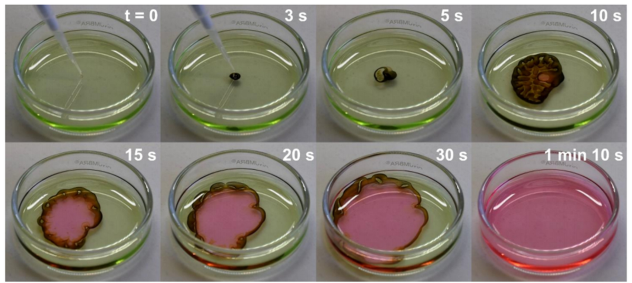
\includegraphics[scale=0.45]{figs/IodateIodine.png}
		\caption{\label{fig:iodateiodine}
		A drop of an iodine solution is placed in the an iodate solution. The reaction is 
		autocatalytic with respect to iodine, and a clear chemical front is observed where
		the iodate solution is ahead of the front and the rich iodine solution behind the front.
		Picture is from Panzarasa, \emph{Reaction Kinetics, Mechanisms and Catalysis}, 135:1349 (2022).
		}
	\end{center}
\end{figure}

The reaction rate can be modelled be applying \emph{mass action kinetics} such that
\begin{equation}
	\label{eq:rkcacb}
  r = k'c_Ac_B \, ,
\end{equation}
where $k'>0$ is the (second order) reaction rate coefficient, and $c_A$ and $c_B$ are the
concentration of $A$ and $B$, respectively. The rate of change for A is then
\begin{equation}
\label{eq:dcAdt}
  \frac{\d c_A}{\d t} = k'c_Ac_B \, .
\end{equation}
Let $c_0=c_A+c_B$ be the total concentration and assume this is a constant, then
\begin{equation}
  \frac{\d c_A}{\d t} = k'c_A(c_0 - c_A) \, .
\end{equation}
Allowing for diffusion and dividing with $c_0$ we have 
\begin{equation}
\frac{\partial c}{\partial t} = kc(1-c) + D \frac{\partial^2c}{\partial x^2}  \, ,
\end{equation}
where $c=c_A/c_0$ and $k=k'c_0$. This is the \emph{Fisher-Kolmogorov equation} or 
\emph{logistic growth with diffusion}. Notice that $c$ is bounded, $0 \leq c \leq 1$.

\begin{question}
	How did we arrive at Eq. (\ref{eq:dcAdt}) from Eq. (\ref{eq:rkcacb})?
\end{question}


Envision that we have a one dimensional system (i.e., a thin tube) 
composed of only reactive B molecules (and likely also an inert solvent). At time $t=0$
we introduce some A molecules at the left boundary, $x=0$. Encounters between A and B
molecules result in the autocatalytic production of A, leading to a local concentration
gradient and, hence, a flux where A molecules diffuse into rich B regions (positive $x$-direction),
where, again, A molecules are produced, and so forth. This, we may imagine,
leads to a propagating concentration front of A moving through the
system in the positive $x$-direction. Behind the front we have A molecules, and ahead of the front B
molecules; in the front zone both A and B molecules are present which react
according to (\ref{react:FK}). This is illustrated in Fig. \ref{fig:fronts}(a). 

One research question we now seek to answer is: \emph{If} the propagating front exists
and \emph{if} the speed is constant, how fast will the front propagate?

\begin{figure}
  \begin{center}
    \includegraphics[scale=0.4]{figs/FK-wavefront}
    \caption{\label{fig:fronts}
	  Propagating front in the standard (or fixed) coordinate system, (a), and in the
	  moving frame coordinate system, (b). The arrow in (a) indicates the direction of the 
	  front propagation (positive $x$-direction).
    }
  \end{center}
\end{figure}

Assume that (after a transient time) the front propagates with a
constant speed, $s$. We can then choose to shift the coordinate system 
with the front speed. In this moving frame the concentration profile is
independent of time. (Imagine you 'sit' on the front moving along with it, 
then you observe it being independent of time. This is not the case for an observer 
standing in a fixed coordinate system, where the front will pass her 
at some point in time.) Since the front propagates in the positive $x$-direction 
we define the moving frame coordinate by
\begin{equation}
  z = x - st \, .
\end{equation}
The concentration profile can now be written as being depended on $z$; 
$c(z)= c(z(x,t))=c(x,t)$. See Fig. \ref{fig:fronts} (b). Importantly, we must expect 
from our basic knowledge of dynamical systems that
\begin{equation}
  \lim_{z \rightarrow -\infty} c = 1  \ \text{and} \   \lim_{z \rightarrow
    \infty} c = 0 \, .
\end{equation}
This means that $c=1$ is an unstable fixed point and that $c=0$ is a stable fixed point. 

In our treatment here, we will require that for a front to exist there must be a $z_0$ such that
\begin{eqnarray}
	\left.\frac{\d c}{\d z} \right|_{z=z_0} \neq 0 
	\ \text{and} \ 
	\lim_{z \rightarrow \pm \infty} \frac{\d c}{\d z} = 0 \, .
\end{eqnarray}
To proceed we need to derive the dynamical equation for the concentration in the 
moving coordinate system. From the chain rule
\begin{equation}
  \frac{\partial c}{\partial t} = -s \frac{\d c}{\d z} \ \
  \text{and} \ \
  \frac{\partial^2 c}{\partial x^2} = \frac{\d^2 c}{\d z^2} \ . 
\end{equation}
Substitution into the Fisher-Kolmogorov equation gives 
\begin{equation}
  \label{eq:fkmvframe}
  D\frac{\d^2c}{\d z^2} + s\frac{\d c}{\d z} + kc(1-c) = 0 \, .
\end{equation}
Remember that $k>0$ since $k'>0$. 

This is an important result: As with the diffusion equation, we have managed to transform a 
partial differential equation into a problem of an ordinary differential equation. 
This is extremely helpful because we can now analyse this using
standard techniques. Also notice that $s$, which we hope to say something
about, enters the problem. 

In our analysis of the dynamics we start with a simple linear stability
analysis. First, we recast the second order differential equation into a system of first order equations 
\begin{eqnarray}
  \frac{\d c}{\d z} &=& v \nonumber \\
  D\frac{\d v}{\d z} &=& -sv - kc(1-c) \, .
\end{eqnarray}
where $v$ is an auxillary variable. The fixed points are 
\begin{equation}
  (c, v)=(0,0)  \ \text{and} \   (c, v)=(1,0) \, .
\end{equation}
From the previous discussion we expect that $(0,0)$ is stable and $(1,0)$ is
unstable, but sometimes our expectations will betray us, and we will now show this. 
The general Jacobian matrix is (please, check!)
\begin{equation}
  \mathbf{J} =
  \begin{bmatrix}
    0 & 1 \\
    k/D(c/2-1) & -s/D
    \end{bmatrix} \, .
\end{equation}
For the fixed point (1,0) we have the eigenvalues
\begin{equation}
  \lambda_{1,2}=-\frac{1}{2}\left(
    \frac{s}{D} \pm \sqrt{\left(\frac{s}{D}\right)^2 + \frac{4k}{D}} 
  \right) \, .
\end{equation}
Since $k>0$ and $D>0$, the sum under the square root is positive and the square root term is 
larger than $s/D$. This means that the eigenvalues are real, one being negative and one positive.
The point (1,0) is then an unstable saddle point. 

For the fixed point (0,0) we have the eigenvalues
\begin{equation}
  \lambda_{1,2}=-\frac{1}{2}\left(
    \frac{s}{D} \pm \sqrt{\left(\frac{s}{D}\right)^2 - \frac{4k}{D}} 
  \right) \, .
\end{equation}
The three possible scenarios are 
\begin{enumerate}
	\item{
			If $(s/D)^2>4k/D$, then the sum under the square root is positive and  
			$\left[\left(\frac{s}{D}\right)^2 - \frac{4k}{D}\right]^{1/2} < s/D$, that is, the eigenvalues are 
			both real and negative; the fixed point is a stable node. 
		}
	\item {
			If $(s/D)^2=4k/D$ we have repeated eigenvalues $\lambda_{1,2}=-2s/D$ and the 
			fixed point is a stable node.
		}
	\item {
			If $(s/D)^2 < 4k/D$ the fixed point has two complex conjugated eigenvalues with negative 
			real parts, that is, the fixed point is a stable spiral.
		}
\end{enumerate}
The last scenario is problematic when we interpret the function $c$ as being a normalized concentration since we then 
require $c \geq 0$. Recall,  $c(z)=c(x,t)=c_A/c_0 \geq 0$. If (0,0) is a stable spiral the 
phase plane trajectories will spiral around the origin (0,0) and $c$ will take negative values. Therefore, the eigenvalues 
cannot be complex, implying that only scenario 1 and 2 are useful. This in turn defines a minimum allowed speed, because 
\begin{equation}
\left(\frac{s}{D}\right)^2 \geq \frac{4k}{D} \ \Rightarrow s \geq 2\sqrt{kD} = s_\text{min}
\, .
\end{equation}
In Fig. (\ref{fig:minspeed}) the trajectories are shown for $s<s_\text{min}$ (the stable spiral case) 
and $s=s_\text{min}$ (the stable node case). 

\textit{Important} From the linear stability analysis we have only derived a minimum allowed
front propagation speed, not the actual speed the front takes. 
This is, furthermore, under the assumption that the front exists and propagates with constant speed. 
To investigate the system further we will rely on numerical analysis, see Exploration \ref{exploration:fisherKol}. 

\begin{figure}
\begin{center}
\includegraphics[scale=.4]{figs/minspeed}
\caption{\label{fig:minspeed} Two phase plane trajectories starting close to
	  the unstable saddle point (1,0). The  
	two examples are when $s = s_\text{min}$ and when $s < s_\text{min}$.
}
\end{center}
\end{figure}

We can do a bit more. Again, we will assume that the front exists and that it propagates with constant speed. 
Now, Eq. (\ref{eq:fkmvframe}) is a non-linear problem, which we cannot solve in general. However, we can find an 
approximate solution using a perturbation method. To this end, we identify a small perturbation parameter 
$\epsilon = 1/s^2$, that is, we focus our analysis on the limit of large front speeds. 
The choice of perturbation parameter is clear when we perform a second coordinate transformation  
\begin{equation} 
\xi = k z \sqrt{\epsilon} \, .
\end{equation}
From the chain rule we have the following identities
\begin{eqnarray}
	\frac{\d c}{\d z} = k\sqrt{\epsilon} \frac{\d c}{\d \xi} \ \ \text{and} \ \  
	\frac{\d^2 c}{\d z^2} = k^2 \epsilon \frac{\d c^2}{\d \xi^2} \, .
\end{eqnarray}
Substituting into Eq. (\ref{eq:fkmvframe}), we get
\begin{equation}
	\label{eq:fkinz}
\epsilon k D\frac{\d^2c}{\d \xi^2} + \frac{\d c}{\d \xi} + c(1-c) = 0 \, .
\end{equation}
This is a singular perturbation problem, since the case
$\epsilon=0$ yields a first order differential equation, which in general is
qualitatively different from the original differential equation. We boldly attempt to continue using the 
(naive) outer solution which we introduced for regular perturbation problems. 

We substitute the Poincar\'{e} expansion 
\begin{eqnarray}
	c(\xi) \sim \sum_{n=0}^N \epsilon^n c_n(\xi)
\end{eqnarray}
into Eq. (\ref{eq:fkinz}) and collect term wise. To zero'th order we obtain
\begin{equation}
\frac{\d c_0}{\d \xi} + c_0(1-c_0)=0 \, .
\end{equation}
This is a first order equation and, also, note it does not contain the diffusion
coefficient. This implies that we look at the effect of the reaction only, but
under the assumption that the front actually exists, hence, the diffusion process is 
implicitly included. Separation of variables gives
\begin{equation}
\frac{\d c_0}{c_0(1-c_0)} = \d \xi \, .
\end{equation}
\begin{wrapfigure}{R}{0.35\textwidth}
	\centering
	\includegraphics[width=0.3\textwidth]{figs/fku0.eps}
%	\caption{\label{fig:bacteriaindish} A figure.}
\end{wrapfigure}
\paragraph{}
\vspace*{-\parskip}
The fraction on the left-hand side can be written as
\begin{eqnarray}
	\frac{1}{c_0(1-c_0)} = \frac{1}{c_0} + \frac{1}{1-c_0} \, ,
\end{eqnarray}
and integration along some re-arrangement gives
\begin{equation}
	c_0 = \frac{1}{1+Ke^{\xi}} \, .
\end{equation}
We choose the IC $c_0(0)=1/2$ giving $K=1$ and therefore
\begin{equation}
c_0 = \frac{1}{1+e^{\xi}} = \frac{1}{1+e^{kz/s}} \, .
\end{equation}
This choice of IC is not unique; different choices will just shift the 
concentration profile in $\xi$-direction. If $s=s_\text{min}$ we get
\begin{equation}
\label{eq:u0fk} 
c_0 = \frac{1}{1+e^{\sqrt{k/(4D)}z}} \, .
\end{equation}
We continue the analysis in the exercises.

The idea of propagating fronts is used to model different systems. Let us see a two-species 
predator-prey example. 
\begin{example}\label{example:multifront}
	This example is from Murray, \textit{Mathematical Biology}; I will leave out 
	quite a few details and recommend that you to following along with pen and paper. 

	We consider predator movement from highly
	populated region of predators into low populated regions. The latter region is
	rich on prey due to the low predator concentration. This version of the model
	assumes that the prey does not perform any migration. Let
	$0 \leq c_1 \leq 1$ be the dimensionless prey concentration and
	$0 \leq c_2 \leq 1$ the dimensionless predator concentration. The model in 
	dimensionless form reads
	\begin{equation}
		\label{eq:pp0}
		\frac{\partial c_1}{\partial t} = c_1(1-c_1-c_2) \ ,
		\ \frac{\partial c_2}{\partial t} =
		ac_2(c_1-b) + \frac{\partial^2 c_2}{\partial x^2} \, ,
	\end{equation}
	where the model parameters follow that $a,b > 0$. 

	We assume that there exists a front and that the front speed is
	constant. We may once more ask the question ``If the front exists, what is the minimum allowed 
	propagation	speed?''. We approach the problem exactly as we did for the Fisher-Kolmogorov
	front, but, just for fun, in this example we let the front propagate from
	right to left (i.e, negative $x$-direction). This means that the moving frame coordinate is given by
	\begin{equation}
	z = x + st \, .
	\end{equation}
	Let $c_1(z)=c_1(x,t)$ and $c_2(z)=c_2(x,t)$. Then in the co-moving frame we have
	the dynamics
	\begin{eqnarray}
		s\frac{\d c_1}{\d z} &=& c_1(1-c_1-c_2) \\ 
		s\frac{\d c_2}{\d z} &=& ac_2(c_1-b) +\frac{\d^2c_2}{\d z^2} 
	\end{eqnarray}
	from which we can form a system of first order differential equations 
	\begin{eqnarray}
	\frac{\d c_1}{\d z}&=& \frac{c_1}{s}(1-c_1-c_2) \nonumber \\
	\frac{\d c_2}{\d z} &=& w  \label{eq:multifrontord}\\
	\frac{\d w}{\d z} &=& sw - ac_2(c_1-b)  \nonumber
	\end{eqnarray}
	Again, $w$ simply acts as an auxillary variables. The fixed points for this are 
	\begin{eqnarray}
		\text{unstable point}:  && (c_1,c_2,w)=(0,0,0) \nonumber \\
		\text{unstable point}: && (c_1,c_2, w)=(1,0,0) \nonumber \\
		\text{stable point}:  && (c_1,c_2,w)=(b,1-b,0) \nonumber 
	\end{eqnarray}
	The first fixed point is simply the trivial case, and is not interesting here. 
	The two other points are more informative:	As $z \rightarrow - \infty$ we approach the unstable fixed point (1,0,0), 
	that is, there is only prey ahead of the front. As $z \rightarrow \infty$ we approach the stable fixed 
	point $(b, 1-b, 0)$, this is the co-existence state between the prey and predator, having 
	concentrations $b$ and $1-b$, respectively. See illustration in Fig. \ref{fig:pp}.
	\begin{figure}
	\begin{center}
	  \includegraphics[scale=0.3]{figs/twospecies.eps}
	\end{center}
	\caption{\label{fig:pp} Illustration of the propagating front system in
		Example \ref{example:multifront}. Front propagation in the fixed frame is 
		indicated by the arrow. $b=2/3$}
	\end{figure}

	We demand that the concentrations are positive and bounded so $0 \leq c_1,c_2 \leq 1$. 
	We can then attempt the	same analysis as we did for the Fisher-Kolmogorov system, 
	but this time for the unstable fixed point (1,0,0). The Jacobian here reads 
	\begin{equation}
	\mathbf{J}(1,0,0) =
	\begin{bmatrix}
	  -1/s & -1/s & 0 \\
	  0 & 0 &1 \\
	  0 & a(b-1) & s
	\end{bmatrix}
	\end{equation}
	giving the three eigenvalues
	\begin{equation}
		\lambda_1 = -\frac{1}{s} \ \ \lambda_{2,3}=\frac{1}{2} \left(
		s \pm \sqrt{s^2 + 4a(b-1) }	\right)
	\end{equation}
	As we seek real eigenvalues, the minimum allowed speed is given by
	$s_\text{min} = 2\sqrt{a(b-1)}$.
\end{example}

\begin{question}
How can we interpret the reaction terms in Eq. (\ref{eq:pp0}) in context of a
predator-prey system? What is the biological interpretation of the parameters
$a$ and $b$?
\end{question}

\begin{exerciseregion}

	\begin{exercise}
		Perform a perturbation analysis of the Fisher-Kolmogorov front up to first
		order in $\epsilon$; you can express $c_1$ in terms of $c_0$. Hint: 
		(i) First, show that $1-2c_0=-c{''}_0/c{'}_0$. (ii) Then show that equation for the 
		first order term is
		\[
			\frac{\d c_1}{\d \xi} - \frac{c{''}_0}{c'_0}c_1 = -kD \frac{\d^2c_0}{\d \xi^2} \, .
		\]
		(iii) Solve this using the general identity from calculus
		\[
			\int \frac{f'(x)}{f(x)} \, \d x = \ln|f(x)| \, .
		\]
		(iv) Finally, use the intial value $u'_0(0)=1/4$ to find the particular solution.
	\end{exercise}

	\begin{exercise} \label{ex:checku0}
		Compare the zero'th order perturbation result, Eq. (\ref{eq:u0fk}), with
		numerical results for different front speeds. 
	\end{exercise}

	\begin{exercise}	
		Recall, our requirements for a front to exist. Can the linear problem
		\begin{eqnarray}
			\frac{\partial c}{\partial t}= c + \frac{\partial^2c}{\partial x^2}
		\end{eqnarray}
		feature a front? 
	\end{exercise}
	
	\begin{exercise}
		Through linear analysis of Eq. (\ref{eq:multifrontord}), show that the two-species 
		predator-prey model can feature (fascinating) oscillatory concentrations in the 
		front zone for certain choice of parameters.
	\end{exercise}

	\begin{exercise}
		In Example \ref{example:multifront}	the predator featured mobility. Will the model 
		support a propagating front if the predator is immobile, but the prey is mobile? 
		Model the mobility with a simple Fickian law.
	\end{exercise}

	\begin{exploration}
		\label{exploration:fisherKol}
		One main result from our study of the Fisher-Kolmogorov front is that
		$s > s_\text{min} = 2\sqrt{kD}$. As stated in the text, we do not know
		\emph{if} such front exists, and if so \emph{what} $s$ actually is. (We only
		know the minimum speed allowed.) Perform a numerical exploration of the
		system, and confirm whether the front exists (under different ICs). If so
		determine the stable front speed. [Note: Carefully explore the convergence of
		the wave speed.]
	\end{exploration}


	\begin{exploration}
	  The spread of dominant genes is modelled through an extended 
	  Fisher-Kolmogorov wavefront
	  \begin{equation}
		\label{eq:efk}
		\frac{\partial N}{\partial t} = k(N_0-N)N - N + D
		\frac{\partial^2N}{\partial x^2} \, .
	  \end{equation}
	  $N=N(x,t) \geq 0$ represents the dominant gene concentration, $k, N_0$, and
	  $D$ are the rate constant, total gene pool, and diffusion coefficient,
	  respectively. We let $x > 0$ and $t \geq 0$.

	  We assume that Equation (\ref{eq:efk}) allows for a
	  propagating wave with constant speed $s$. 
	  \begin{enumerate}
	  \item Perform a coordinate transformation using $z=x-st$ such that the
		wave is fixed in this coordinate system.
	  \item Show that $N \geq 0$ implies $kN_0 \geq 1$ if the wave front
		exists. What is the constant gene concentration behind the front?
	  \item Show that the minimum allowed speed is 
		$s_{\text{min}}=2\sqrt{D(kN_0-1)}$ if the front exists.
	  \item Perform numerical simulations confirming the results
		above. Describe what happens when $k=1$ $D=1$ and $N_0=0.5$
		(ignoring coefficient units). Clearly state your choice of boundary
		conditions.
	  \end{enumerate}
	\end{exploration}
\end{exerciseregion}


\section{Turing structures}
Recall Example \ref{example:turing}; in this section we will explore 
how these \emph{diffusion driven spatial structures} emerge in reaction-diffusion systems. 
At first thought, the existence of apparently spontaneously formed
structures contradict our intuition about diffusion processes which tend to reduce and eventually remove the gradients.  
However, for multi-variable systems and for certain types of reactions  
structures emerge and they can even be stable forming static structures with permanent  
spatial concentration gradients. The structures were first found theoretically by 
\emph{Alan Turing}\footnote{Whom, by the way, is also famous for inventing the 
Turing machine and cracking the Enigma code during the second world war.} in the early 1950s, 
which is why they also bare his name. 

We will here explore the Turing structures through the \emph{FitzHugh-Nagumo (FHN) model} 
used to study different excitable systems. For example, 
it is the standard model for a neuron electrical signal (also called neuron firing) caused 
by voltage build-up and release. A simple version of the model is 
in the homogeneous case (where we can ignore diffusion)
\begin{eqnarray}
	\label{eq:fhn1}
	\frac{\d c_1}{\d t} &=& c_1 - c_1^3 - c_2 + \alpha = r_1\\
	\label{eq:fhn2}
	\frac{\d c_2}{\d t} &=& \beta(c_1 - c_2) = r_2
\end{eqnarray}
where $c_1$ is the voltage and $c_2$ acts as a coarse grained variable that describes the 
coupling between the voltage and other relevant cell mechanisms. Notice, the function definitions 
of $r_1$ and $r_2$ on the right-hand; they will be used below. 
The model parameters fulfill $\alpha, \beta > 0$. For now, we will not go into a 
more detailed bio-physical interpretation of the model, and right away
start the mathematical analysis. 

t is easy to verify that there exists a single fixed point, namely, 
\begin{equation}
	(\alpha^{1/3}, \alpha^{1/3}) = (a, b)\, .
\end{equation}
Notice that we will use the symbols $a$ and $b$ for the fixed point coordinates; this is just 
to ease and clarify the reading a bit. It is worth to recapture some of the details in the standard 
linear analysis: We first linearise the dynamical equations in a neighbourhood 
around the fixed point $(a,b)$. For $r_1$ we have
\begin{eqnarray}
	r_1 &=& r_1(a,b) + \frac{\partial r_1}{\partial c_1}(c_1-a) + \frac{\partial r_1}{\partial c_2}(c_2-b) + \ldots \\
				 &=&	(1-3a^2) u - v + \dots
\end{eqnarray}
where $u$ and $v$ describe the deviation of $c_1$ and $c_2$ to the fixed point
\begin{equation}
	u = c_1 - a \ \ \text{and} \ \ v = c_2 - b \, .
\end{equation}
For $r_2$ we have 
\begin{equation}
	r_2 = \beta u - \beta v + \ldots
\end{equation}
We can now readily write the Jacobian in the fixed point 
\begin{equation}
\matrx{J} = 
	\begin{bmatrix}
    1-3\alpha^{2/3} & -1 \\
    \beta & -\beta
 \end{bmatrix} \, ,
\end{equation}
and the eigenvalues are found from the characteristic polynomial
\begin{equation}
	\lambda^2 + (\beta-1+3\alpha^{2/3})\lambda + 3\beta\alpha^{2/3} = 0 \, .
\end{equation}
Without loosing the main conclusions we choose $\alpha$ such that $\alpha^{2/3}=1/10$; 
in this case the eigenvalues are 
\begin{equation}
	\lambda_{1,2} = \frac{1}{2}\left(
	\frac{7}{10}-\beta \pm \sqrt{\beta^2-13\beta/5+49/100} 
	\right) \, .
\end{equation}
We see that the eigenvalues are complex (and conjugate) 
whenever $\beta^2-13\beta/5+49/100<0$ implying that in the interval
\begin{eqnarray}
	\frac{1}{10}\left(13 - \sqrt{120}\right) < \beta <  \frac{1}{10}\left(13 + \sqrt{120}\right) 
\end{eqnarray}
the system features oscillatory behaviour. 

In this interval the real part of the eigenvalues also
changes sign indicating that a bifurcation occurs ($\beta$ being the bifurcation parameter). 
A bit more formally, we expect a bifurcation at $\beta=7/10$, where 
$\text{Re}(\lambda_{1,2})=0$ and where 
\begin{eqnarray}
	\frac{\d\text{Re}(\lambda_{1,2})}{\d \beta} = -1/2 \neq 0 \, .
\end{eqnarray}
This last property is \emph{the transversal condition} which ensures 
that the eigenvalue real part, in fact, changes sign. Thus, we have 
\begin{description}
	\item[$(13 - \sqrt{120})/10 < \beta < 7/10$]{The fixed point is an unstable spiral point}
	\item[$\beta = 7/10$]{The fixed point is non-hyperbolic (the stability is unknown from the linear analysis)}
	\item[$7/10 <\beta < (13 + \sqrt{120})/10$]{The fixed point is a stable spiral.}
\end{description}
This indicates a \emph{Hopf bifurcation} at $\beta = 7/10$: 
(i) For $\beta < 7/10$ the solution converges to a stable \emph{limit cycle}, 
i.e, the system has sustained oscillations (with respect to time) 
below the bifurcation parameter value. See Fig. \ref{fig:fhnbif}. 
(ii) For $\beta > 7/10$ the oscillations are dampened 
and the system relaxes to the stable fixed point. 
Both the condition $\text{Re}(\lambda_{1,2})=0$ and the transversal 
condition are necessary, but not sufficient, conditions for a Hopf bifurcation. 
\begin{figure}
  \begin{center}
    \includegraphics[scale=.45]{figs/fhnPhasePortrait.eps}
    \caption{
    \label{fig:fhnbif} Phase plane trajectories for the FHN model system. 
	  Left: $\beta < 7/10$. Right: $\beta>7/10$.
		Fixed point illustrated by the filled circle. 
		Trajectories are obtained from numerical solutions.
    }
  \end{center}
\end{figure}


We now include diffusion for both $c_1$ and $c_2$ and show that if the diffusion coefficients 
are different, $D_1 \neq D_2$, the system can be unstable in the parameter interval 
$7/10 <\beta < (13 + \sqrt{120})/10$ and $\alpha^{2/3} = 1/10$, 
that is, in the interval where the homogeneous case is stable.  

Again we perform a linear stability analysis, but this time for the full RD-equation. 
First we note that 
\begin{equation}
	\frac{\partial c_1}{\partial t} = \frac{\partial u}{\partial t} \ \ \text{and} \ \ 
	\frac{\partial^2 c_1}{\partial x^2} = \frac{\partial^2 u}{\partial x^2}
\end{equation}
and so forth for the derivatives of $c_2$ and $v$. Then we can write the linearized 
RD-equations in terms of $u$ and $v$, i.e, in terms of the deviation from the homogeneous fixed point
\begin{eqnarray}
	\label{eq:fhnlin1}
	\frac{\partial u}{\partial t} &=& (1-3\alpha^{2/3})u - v + D_1 \frac{\partial^2 u}{\partial x^2}\\
	\label{eq:fhnlin2}
	\frac{\partial v}{\partial t} &=& \beta(u-v) + D_2 \frac{\partial^2 v}{\partial x^2}
\end{eqnarray}
with $D_1$ and $D_2$ being the usual diffusion coefficients. The boundaries we apply here are the zero Neumann BCs 
\begin{equation}
	\left.\frac{\partial u}{\partial x}\right|_{x=0} = \left.\frac{\partial u}{\partial x}\right|_{x=L} = \left.\frac{\partial v}{\partial x}\right|_{x=0} = \left.\frac{\partial v}{\partial x}\right|_{x=L} = 0 \, .
\end{equation}
The initial condition is such that the spatial average of $u$ and $v$ are zero, that is, with some $u$ and $v$ are randomly distributed around the
point $(a,b)$ with sufficiently small amblitude. 

From our earlier experience with the linear RD-equation under Neumann BCs 
we expect that the solutions for $u$ and $v$ are cosine Fourier series, that is,
\begin{equation}
\label{eq:turingguess}
	u(x,t) = \sum_{n=1}^\infty u_n e^{\lambda_n t}\cos\left(\frac{n\pi}{L} \, x\right) \ \ \text{and} 
	\ \ v(x,t) = \sum_{n=1}^\infty v_n e^{\lambda_n t}\cos\left(\frac{n\pi}{L} \, x\right) \, . 
\end{equation}
We do not know $\lambda_n$, that is, in our proposition the temporal dynamics is still undetermined. 
Now, the solutions must of course fulfill the two linearized equations. Thus, 
substituting the guess, Eq. (\ref{eq:turingguess}), into Eq. (\ref{eq:fhnlin1}) and differentiating we get
for each term, $n$, we have
\begin{eqnarray}
	\lambda_n u_n e^{\lambda_n t} \cos\left(\frac{n\pi}{L} \, x\right) 
	&=& \frac{7}{10}u_n e^{\lambda_n t} \cos\left(\frac{n\pi}{L} \, x\right)  \nonumber \\
	&-& v_n e^{\lambda_n t} \cos\left(\frac{n\pi}{L} \, x\right) 
	- D_1 u_n \left(\frac{n\pi}{L}\right)^2 e^{\lambda_n t} \cos\left(\frac{n\pi}{L} \, x\right)
	\nonumber \\
\end{eqnarray}
using the value $\alpha^{2/3}=1/10$. The exponential terms cancels, and if we rearrange we obtain
\begin{equation}
	\left(
		\lambda_n u_n -\frac{7}{10} u_n + v_n + \left(\frac{n\pi}{L}\right)^2 u_n D_1
	\right) \cos\left(\frac{n\pi}{L} \, x\right) = 0 \, . 
\end{equation}
Repeating this for Eq. (\ref{eq:fhnlin2}) we get the identity 
\begin{equation}
	\left( \lambda_n v_n - \beta u_n + \beta v_n + \left(\frac{n\pi}{L}\right)^2 v_n D_2
	\right) \cos\left(\frac{n\pi}{L} \, x\right) = 0 \, .
\end{equation}
We can combine these two equations and obtain a more convenient (and hopefully recognizable) form. 
First, let $\vec{W}_n = (u_n, v_n)^T$ and recall that the 
diffusion matrix is defined as
\begin{equation}
	\mathbf{D} =
	\begin{bmatrix}
	D_1 & 0 \\
	0 & D_2
	\end{bmatrix}
\end{equation}
then we have on matrix-vector form
\begin{equation}
	\left[
		\lambda_n \matrx{I} - \matrx{J} + \left(\frac{n\pi}{L}\right)^2 \, \matrx{D}
	\right] \cdot \vec{W}_n \cos\left(\frac{n\pi}{L} \, x\right) = \vec{0} \, .
\end{equation}
This, you may see, is an eigenvalue problem. As usual, we do not seek the trivial case 
$\vec{W}_n=\vec{0}$, as this leads to the trivial solutions for $u_n$ and $v_n$. 
A non-trivial solution exists if the matrix
\begin{equation}
	\left[
		\lambda_n \matrx{I} - \matrx{J} + \left(\frac{n\pi}{L}\right)^2 \, \matrx{D}
	\right]
\end{equation}
is rank deficient, that is, if there exists one or two $\lambda_n$ such that the determinant is zero
\begin{eqnarray}
\label{eq:turingeig}	
	\mbox{} & \left|
		\lambda_n \matrx{I} - \matrx{J} + \left(\frac{n\pi}{L}\right)^2 \, \matrx{D}
	\right| = 
	\left(
		\lambda_n - \frac{7}{10} +\left(\frac{n\pi}{L}\right)^2 D_1
	\right) 
\left(
	\lambda_n + \beta +\left(\frac{n\pi}{L}\right)^2 D_2
	\right) + \beta = 0  \, . \nonumber \\
\end{eqnarray}
Before solving this quadratic problem, we introduce the two auxiliary variables 
\begin{eqnarray}
	a_n = -\frac{7}{10} + k^2 D_1, \text{and} \  \
	b_n = \beta + k^2 D_2
\end{eqnarray}
where $k=n\pi/L$ is the wave vector. The solution can now be written as 
\begin{eqnarray}
	\lambda_{n,1,2} = \frac{1}{2}\left( 
		-(a_n+b_n) \pm \sqrt{(a_n+b_n)^2 - 4(\beta + a_nb_n)}
	\right) \, .
\end{eqnarray}
Notice that the eigenvalues are functions of $n, \beta, D_1$, and $D_2$. 

We can know investigate the dynamics for each Fourier term (or Fourier mode): 
If the real part of the eigenvalue is negative for a given mode
this mode is stable, whereas if the real part is positive the mode is unstable. As always, in case 
of zero real part (the non-hyperbolic case) we cannot conclude anything about the stability of 
the system. Figure \ref{fig:dispersion} shows the real part of the eigenvalues $\lambda_{n}$ 
as function of wave vector, which is equivalent to a plot of the real part of 
$\lambda_n$ versus $n$. This is the \emph{dispersion plot}, 
and the eigenvalue's dependency on $k$ is called a \emph{dispersion relation}. We have used 
$D_2 = 10D_1$ and $\beta=1$. 
\begin{figure}
	\begin{center}
    \includegraphics[scale=.3]{figs/dispersion}
    \caption{
		\label{fig:dispersion} Dispersion plot: Real part of the eigenvalues, $\lambda_{n}$ 
		as a function of $k=n\pi/L$. $D_2 = 10 D_1$, $\alpha = (1/10)^{3/2}$, and $\beta = 1$. 
	}
  \end{center}
\end{figure}
Some of the Fourier modes (indicated by the blue interval) are unstable, hence, the  
solution to the linearized system, Eq. (\ref{eq:turingguess}), grows exponential in time and the 
system is unstable. 

This is a linear analysis. The non-linear part of the system may eventually 
suppress this growth as $u$ and $v$ become sufficiently large and thus form a 
steady state structure. 

We can solve the non-linear RD-equation using the FTCS algorithm. We will do this using 
the same parameter values as in
Fig. \ref{fig:dispersion}. The voltage $c_1$ is plotted as function of $x$ for four different times 
in Fig. \ref{fig:turingfhn}. It is seen that the structure emerge from the homogeneous state reaching a 
final steady state. 
\begin{figure}
  \begin{center}
    \includegraphics[scale=.3]{figs/turingfhn}
    \caption{
		\label{fig:turingfhn} 
		FHN model voltage profiles as function of $x$ for four different times. 
		Black line is the condition. Red and green lines are 
		transient profiles, and blue is the final steady state profile. 
		Parameter values are the same as in Fig. \ref{fig:dispersion}.
    }
  \end{center}
\end{figure}
An important observation from the numerical simulations is that the (characteristic) period of the 
structure is given by
\begin{eqnarray}
	p = 2\pi/k_\text{max} \, .
\end{eqnarray}
$k_\text{max}$ is also shown in Fig. \ref{fig:dispersion}. This means that the Fourier mode with largest 
eigenvalue (real part) grows the fastest and dominates the final steady state. 
Again, this is all based on the linear analysis and not some thing we can conclude in general. 

We end this section by listing three necessary conditions for a system to feature 
diffusion-driven instabilities (or Turing structures). 

\begin{theorem}
	\label{th:turing}
	Consider a two species RD-equation with equilibrium point $(a,b)$ and Jacobian
	\begin{eqnarray}
		\mathbf{J}(a,b) = 
		\left[	\begin{matrix}
			a_{11} & a_{12} \\
			a_{21} & a_{22}
		\end{matrix}
		\right]
	\end{eqnarray}
	\emph{If} the system feature Turing structures then
	\begin{enumerate}
		\item $a_{11} a_{22} < 0 $
		\item $a_{12} a_{21} < 0 $
		\item $D_1 \neq D_2$.
	\end{enumerate}
	We will not proof this theorem.
\end{theorem}

\begin{exerciseregion}
	\begin{exercise}
		For the FitzHugh-Nagumo model use $D_1=1, \alpha=(1/10)^{3/2}, \beta=2$, and $L=200$. 
		Find the values for $D_2$ and corresponding wavenumbers $n$, where unstable Fourier modes emerges. 
		Predict the wavelength, and confirm your findings from numerical simulations of the RD-eq system.
	\end{exercise}
	\begin{exercise}
		Theorem \ref{th:turing} limits the possibilities of signs the Jacobian matrix elements can have. Illustrate 
		this by writing the Jacobian with the elements sign only. (This leads to two concepts, namely, 
		\emph{activator-inhibitor} and \emph{positive feedback}. 
	\end{exercise}
	\begin{exercise}
		Recall the Lotka-Volterra predator-prey model 
		\begin{eqnarray}
			\frac{\d c_1}{\d t} &=& c_1 - c_1c_2 \nonumber \\
			\frac{\d c_2}{\d t} &=& c_1c_2 - \alpha c_2
		\end{eqnarray}
		with $\alpha>0$ and $c_1,c_2 \geq 0$. 
		Does the corresponding RD-equation allow for diffusion-driven instabilities?
	\end{exercise}
	\begin{exploration}
		We consider the RD-equation system
		\begin{eqnarray}
			\frac{\partial c_1}{\partial t} = \frac{c_1^2}{c_2} - b c_1 + \frac{\partial^2 c_1}{\partial x^2} \\
			\frac{\partial c_2}{\partial t} = c_1^2 - c_2 + D \frac{\partial^2 c_2}{\partial x^2}
		\end{eqnarray}
		Determine the fixed point for $c_1, c_2 > 0$ in the homogeneous case. 
		Then determine critical value for $b$, where this fixed point is stable. 
		Now, choose $b=0.5$, and find the dispersion curve for different values of $D$; identify the range of 
		possible unstable Fourier modes on the curve. Based on this analysis, explore numerically 
		whether Turing structures 
		exists or not. (Inspired by Murray, \textit{Mathematical Biology}.) 
	\end{exploration}
	
\end{exerciseregion}






%\clearpage


%\begin{appendices}
%\appendixpage
%\noappendicestocpagenum
%\addappheadtotoc
\chapter{Appendices}

%\documentclass[11pt]{article}

%\usepackage{amssymb}
%\usepackage{graphics}
%\usepackage{graphicx}
%\usepackage{pstricks}
%\usepackage{amsbsy}
%\usepackage{amsmath}
%\usepackage{amssymb}

%\newcommand{\R}{\mathbb{R}}
%\newcommand{\bigo}{\mathcal{O}}

%\newcounter{exploration}
%\newenvironment{exploration}[1][]{\refstepcounter{exploration}\par\medskip\noindent%
%  \textbf{Exploration~\theexploration. #1}\rmfamily}{$\square$ \medskip}
   
%\title{Numerical exploration: Slow Fourier transform}
%\date{}
%\author{J.S. Hansen}

%\begin{document}


%\maketitle

\section{The slow Fourier transform (SFT)} \label{appendix:fourier}
Recall that the Fourier coefficients for a function $f$ are given by
\begin{eqnarray}
  a_n &=& \frac{1}{L}\int_{-L}^L f(x) \cos(n\pi x/L) \, dx \\
  b_n &=& \frac{1}{L}\int_{-L}^L f(x) \sin(n\pi x/L) \, dx 
\end{eqnarray}
These two integrals are on the general form
$\int_{-L}^L g(x) dx$. Now, integrals can be quite a mouthful, and
it is therefore useful to device a numerical and therefore approximative method.

The geometrical interpretation of an integral for a function
$g: \R \supseteq D \rightarrow \R$ is the area between the first axis
and the graf of $g$ (with sign!). The area can be approximated by
rectangles; this is also the fundamental idea behind both Riemann and
Darboux definitions of the integral. Figure \ref{fig:trapz}
illustrates how a set of rectangular areas $A_1, A_2, \ldots $
approximates the integral of $g$ in the interval
$x_0 \leq x \leq x_N$.
\begin{figure}[h]
  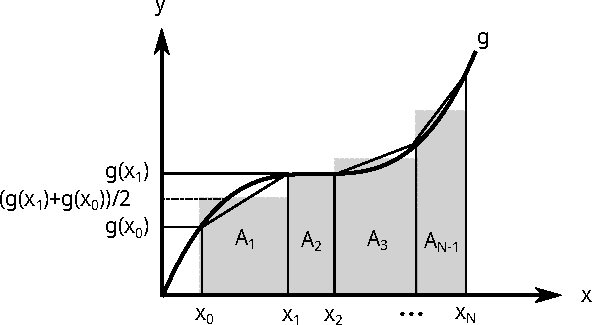
\includegraphics[scale=1.0]{figs/trapz.pdf}
  \caption{\label{fig:trapz}Illustration of the trapzoidal rule}
\end{figure}
Each area is 
\begin{equation}
  A_i = (x_i - x_{i-1}) \frac{g(x_i)+ g(x_{n-1})}{2}
\end{equation}
and we hope that
\begin{equation}
  \int_{x_0}^{x_N} g(x) d x = \lim_{n \rightarrow \infty} \sum_{i=1}
  ^n A_i \, .
\end{equation}
This is the trapzoidal rule.

\begin{exerciseregion}
\begin{exercise}
	Implement the trapzoidal rule. Test it against a known integral, for example, 
	$\int_0^{2\pi} \cos(x) \d x$. Explore the trapz rule's precision by changing 
	the sub-interval length $x_i - x_{i-1}$. 
\end{exercise}

\begin{exercise}
  Let $f(x) = -x$, where for $-1 \leq x \leq 1$ such that
  $L=1$. Use your implementation of the trapzoidal rule to
  numerically calculate the Fourier coefficients and compare with the
  analytical result. 
\end{exercise}

\begin{exercise}
  Download the data file \textsf{fourier.dat} from the moodle
  page. How many different Fourier modes can you detect using your code?
\end{exercise}
\end{exerciseregion}

%\end{document}



\section{The FTCS algorithm} \label{sect:ftcs}
%\section{Appendix B}
Before advicing a numerical scheme for the diffusion equation it is
illustrative to first see an example a scalar differential equation, and how this 
can be solved numerically. In particular, it will introduce some of the symbolism we will use 
later.

We consider the general first order problem 
\begin{equation}
  \label{eq:I:difscalar}
  \frac{\d c}{\d t} = c'(t) = f(c, t) \ , \ \ \ c(t_0)=c_0
\end{equation}
such that $c: I \rightarrow \R$, $I \subseteq \R$ and $f$ is known, of course. 
This defines an \emph{inital value problem}; for these problems we usually use $t$ 
as the free variable rather than $x$. 

We assume that the function $c$ can be represented by a  
Taylor series, i.e., by definition $c$ is analytical in all interior points in $I$. (We actually do not need this strict condition, but it will 
save us some headaches.) We then Taylor expand $c$ around an interior point $a \in I$
\begin{eqnarray}
	c(t) = c(a) + c'(a)(t-a) + \sum_{k=2}^\infty   \frac{c^{(k)}(a)}{k!}(t-a)^k \, . 
\end{eqnarray}
We will write this is in a slightly different way by introducing $\Delta t = t -a$
\begin{eqnarray}
  c(a + \Delta t) &=& c(a)+c'(a)\Delta t + \sum_{k=2}^\infty
  \frac{c^{(k)}(a)}{k!}\Delta t^k \nonumber \\ &=&
  c(a)+c'(a)\Delta t + \bigo(\Delta t^2)
\end{eqnarray}
where $\Delta t = t-a$. $\bigo$ is the remainder function (called
big-O) and the argument to $\bigo$ indicates the lowest order in
$\Delta t$, here $\Delta t^2$. Loosely speaking, we say that
$\bigo(\Delta t^{k})$ goes faster to zero than $\bigo(\Delta t^{k-1})$
as $\Delta t$ goes to zero. Re-arranging gives
\begin{equation}
  \label{eq:o1}
  c'(a) = \frac{c(a+\Delta t)-c(a)}{\Delta t} - \bigo(\Delta t)
\end{equation}
using $\bigo(\Delta t^2)/\Delta t = \bigo(\Delta t)$. 
Substitution into the original differential equation, Eq. (\ref{eq:I:difscalar}), and re-arranging 
gives  
\begin{equation}
  c(a+\Delta t) = c(a) + \Delta t f(c(a), a) + \bigo(\Delta t^2) \, .
\end{equation}
To use this in practise we can let $t_0=0$, that is, we have the
initial condition $c(0)=c_0$. Then, we have by substitution
\begin{eqnarray}
  c(\Delta t) &=& c_0 + \Delta t f(c_0, 0) +
  \bigo(\Delta t^2) \nonumber \\
  c(2\Delta t) &=& c(\Delta t) + \Delta t
	f(c(\Delta t), \Delta t) + \bigo(\Delta t^2) \nonumber \\
  &\ldots& \nonumber \\
  c((n+1)\Delta t) &  =& c(n\Delta t) +
  \Delta t f(c(n\Delta t), n\Delta t) + \bigo(\Delta t^2)
  \label{eq:I:iteration} \\
  &\ldots& \nonumber
\end{eqnarray}
This presents an iterative scheme: from $c(0)=c_0$ we evaluate the
function value at $t=\Delta t$, and from this the value at $t=2\Delta
t$, etc. This is the simplest numerical scheme we can compose, and it is called the
\emph{first order forward Euler scheme} or just the Euler scheme.

Usually we replace the argument with the iteration index such that
$c(n \Delta t) = c^n$. Eq. (\ref{eq:I:iteration}) is then
written as (leaving out the $\bigo$-function)
\begin{equation}
  c^{n+1} = c^n + \Delta t f(c^n, n\Delta t)
\end{equation}
The Euler scheme is called an explicit scheme because the
value at time $(n+1)\Delta t$ is given explicitly in terms of values
at time $n\Delta t$. It is important to note that explicit schemes are
so called non-symplectic and they cannot be used to solve problems
where there is a system constant, for example, a constant energy.

\bigskip

\noindent Moving on to the diffusion equation. Recall, for a Dirichelt problem we have 
\begin{equation}
  \frac{\partial c}{\partial t} = \frac{\partial^2 c}{\partial
    x^2}
\end{equation}
with boundary and initial values
\begin{equation}
	c(x,0) = f(x) \ \ \mbox{and} \ \ c(0,t) = c_0 \ \ c(L,
  t) = c_L \, .
\end{equation}
Again $c$ is analytical on its domain, $t \geq 0$, and $0\leq x \leq L$. 

Keeping $x$ fixed we can Taylor expand with respect to $t$ giving
\begin{equation}
  c(x, a+\Delta t) = c(x,a) + \left.\frac{\partial c}{\partial
    t}\right|_{t=a}\Delta t + \bigo(\Delta t^2) \, ,
\end{equation}
or equivalently
\begin{equation}
  \left. \frac{\partial c}{\partial t}\right|_{t=a} = 
  \frac{c(x, a+\Delta t)- c(x,a)}{\Delta t} - \bigo(\Delta t) \, .
\end{equation}
Now, keep $t$ fixed. We Tayler expand up to second order with respect to $x$, thus, 
around a point $0<b<L$ we get 
\begin{equation}
  c(b+\Delta x, t) = c(b,t) + \left.\frac{\partial c}{\partial x}\right|_{x=b}\Delta
  x + \left.\frac{1}{2}\frac{\partial^2 c}{\partial x^2}\right|_{x=b} \Delta x^2 +
  \bigo(\Delta x^3)
  \label{eq:I:2orderf}
\end{equation}
where $\Delta x = x-b$. There is an annoying first order derivative
here; thankfully we can eliminate this by noting that
\begin{equation}
  c(b-\Delta x, t) = c(b,t) - \left.\frac{\partial c}{\partial x}\right|_{x=b} \Delta
  x + \left.\frac{1}{2}\frac{\partial^2 c}{\partial x^2}\right|_{x=b} \Delta x^2 +
  \bigo(\Delta x^3)
   \label{eq:I:2orderb}
\end{equation}
Hence, addition of Eqs.(\ref{eq:I:2orderf}) and (\ref{eq:I:2orderb})
gives
\begin{equation}
  c(b+\Delta x, t) + c(b-\Delta x, t) = 2 c(b,t) + \left.\frac{\partial^2
    c}{\partial x^2}\right|_{x=b} \Delta x^2 + \bigo(\Delta x^4)
\end{equation}
or
\begin{equation}
  \left.\frac{\partial^2 c}{\partial x^2}\right|_{x=b} =
  \frac{c(b+\Delta x, t) - 2 c(b,t) + c(b-\Delta x, t) }{\Delta x^2} -
  \bigo(\Delta x^2) \label{eq:I:secondorder}
\end{equation}
Again, we replace the arguments with iteration index, i.e.,
\begin{eqnarray}
	c(x,t)&=&c_i^n \nonumber \, \\
	c(x,t+\Delta t)&=&c_i^{n+1} \, \nonumber \\ 
	c(b+\Delta x,t)&=&c_{i+1}^n \, \nonumber \\
	c(b-\Delta x,t) &=& c_{i-1}^n \,
	\end{eqnarray}
and we write the diffusion equation as (leaving out the $\bigo$s)
\begin{equation}
\frac{c_i^{n+1} - c_i^n}{\Delta t} \approx \frac{c_{i-1}^n -
  2c_i^n + c_{i+1}^n}{\Delta x^2} 
\end{equation}
readily giving the iterative scheme for point $i$
\begin{equation}
  c_i^{n+1} = c_i^n + \Delta t \left[\frac{c_{i-1}^n -2c_i^n +
    c_{i+1}^n}{\Delta x^2}\right] \, .
\end{equation}
This scheme is called the forward time centered space (FTCS) algorithm
and is also an explicit scheme. 

\begin{exerciseregion}
    \begin{exercise}    
    Consider the differential equation
    \begin{equation}
        \label{eq:expl1}
		c'(t) = 1 - c \ \text{with} \ c(0) = 0
    \end{equation}
	Solve this initial value problem. Then impliment the Euler scheme and solve the
	problem numerically. (Use your favorite programming language; if this
	is Java you are on your own!)  Test your implementation against the
    analytical result.
    \end{exercise}
    
    \noindent Note: The error we make at each time step can be evaluated
    directly from the higher order Taylor polynomial terms if the function
    $c$ is known. Use this fact if you wish.

 \begin{exercise}
  Let $c(x) = 1-x^2$, where $0 \leq x \leq 1$ and $c(0)=c(1)=0$. Use
  Eq. (\ref{eq:I:secondorder}) to calculate the second order
  derivative. Compare to the analytical result. Make a plot of the
  error as function of $\Delta x$.   
\end{exercise}

\begin{exercise}
  Implement the FTCS alorithm. Use this to solve a diffusion problem
  where the analytical solution is known. Discuss possible errors.
\end{exercise}

\end{exerciseregion}


\section{Existence and uniqueness of the RD-equation}
We here list the general criteria for a solution to the RD-equation to exist; 
again we will not prove these criteria, but discuss examples. 

First, we must define Lipschitz continuity: 
A function $f: I \rightarrow \R$ is Lipschitz continuous on the real interval $I$
if there exists a $K \in \R$ such that
\begin{equation}
  |f(x)-f(y)| \leq K |x-y| \ , \ x,y \in I \, .
\end{equation}
This definition basically states that if the function is Lipschitz continuous, the function 
cannot have an infinite rate of change anywhere on its domain. Let see a standard example of 
function, which is \emph{not} Lipschitz continuous.

\begin{example}
	The function $f(x) = \sqrt{|x|}$ is not Lipschitz continuous on the domain $I=[-1,1]$.

	\begin{proof}
		We focus on the likely troublesome point $x=0$; we have from the definition
		\begin{equation}
		    |f(0)-f(y)| \leq K |0-y| \ \Rightarrow \ |f(y)| \leq K|y| \, ,
		  \end{equation}
		that is, for $y \neq 0$ we get 
		\begin{equation}
		    K =\frac{\sqrt{|y|}}{|y|} = \frac{1}{\sqrt{|y|}} \, . \ \ \ \ \ \ (y \neq 0) 
		\end{equation}
		This fraction diverges as $y \rightarrow 0$, hence, $K$ does not exist. 
	\end{proof}

	\noindent Notice that $f$ is continuous in the usual Weierstrass definition 
	and that Lipschitz continuity is in this sense a 
	"stronger" condition on the function than usual continuity. 
\end{example}

We are now ready to list the four criteria that guarantee the existence and
uniqueness of a solution to the RD-equation 
\begin{equation}
  \frac{\partial c}{\partial t} = r(c) + D \frac{\partial^2 c}{\partial x^2}
 \ ,  
\end{equation}
with IC $c(x,0)=f(x)$ and Dirichlet BCs
\begin{equation}
   c(0,t)=c(0,L)=0 \, ,
\end{equation}
or Neumann BCs
\begin{equation}
    \left.\frac{\partial c}{\partial x}\right|_{x=0} = 
  \left.\frac{\partial c}{\partial x}\right|_{x=L} = 0 \ , 
\end{equation}
where  $x \in [0;L]$ and $t \geq 0$. These are (from Allen
\textit{An Introduction to Mathematical Biology}),
\begin{enumerate}
\item{$f(x)$ is continuous on the interior open domain $]0;L[$,}
\item{$f(x)$ has a lower and upper bound, i.e.,
    $\exists \, a,b \, \in \R \, : a\leq f(x) \leq b$ where
    $x \in ]0;L[$,}
\item{the reaction function fulfills $r(a) \geq 0$ and $r(b) \leq 0$, and }
\item{$r$ is Lipschitz continuous on $[0;L]$}
\end{enumerate}
Let us at least see an example.

\begin{example}
  Let us examine the existence and uniqueness for Example
	\ref{example:linearonemode} on page \pageref{example:linearonemode} using $k>0$. (i) $f(x)$
  is continuous for all $x \in ]0;L[$. (ii) Since $0\leq f(x) \leq 1$, $f$
  has a lower and an upper bound. (iii) $r(0) = 0$, but since $r(1) \not\leq
  0$ we are not guarantied a solution. This is consistent with the discussion in
  the example.
\end{example}

\begin{question}
	Are we guarantied a solution for Example \ref{example:linearonemode} if $k<0$?
\end{question}

\begin{exerciseregion}
  \begin{exercise}
    Are we guaranteed a solution to the Fisher-Kolmogorov equation
    \begin{equation}
      \frac{\partial c}{\partial t} = kc(1-c) + D \frac{\partial^2c}{\partial x^2}  
    \end{equation}
	  with zero Neumann BCs if the IC fulfills 
	  $0\leq f(x) \leq 1$ and is continuous on $]0; 1[$? 
  \end{exercise}
\end{exerciseregion}







%\end{appendices}

\end{document}
